\documentclass[14pt, a0paper, landscape, margin=0mm, innermargin=15mm,
   blockverticalspace=15mm, colspace=15mm, subcolspace=8mm]{tikzposter}
\usepackage[T1]{fontenc}
\usepackage{amssymb}
\usepackage{float}
\usepackage[backend=bibtex]{biblatex}
\addbibresource{references.bib}
\setlength{\tabcolsep}{2em}

% title, author, and institution
\title{\fontsize{25pt}{1em} An Explicit, Positive CFEM Scheme Based on FCT}
\author{\begin{tabular}{c c c}
  Jean C. Ragusa       & Jean-Luc Guermond      & Joshua E. Hansel\\
  jean.ragusa@tamu.edu & guermond@math.tamu.edu & joshhansel@tamu.edu\\
  Texas A\&M University & Texas A\&M University & Texas A\&M University
\end{tabular}}

\definebackgroundstyle{mybackground}{
  \node[at=(current page.center)] at (0,0) {
\includegraphics[height=\textheight]{figures/blue_gradient.png}};
}

% theme and style and colors
\usetheme{Autumn} % Default, Rays, Basic, Simple, Envelope, Wave, Board, Autumn, and Desert
\usebackgroundstyle{mybackground} % Default, Rays, VerticalGradation, BottomVerticalGradation, Empty
\usecolorstyle[colorOne=blue,colorTwo=black!10!blue!20,colorThree=blue!90!black]{Russia} % Default, Australia, Britain, Sweden, Spain, Russia, Denmark, Germany
\usetitlestyle{Empty} % Default, Basic, Envelope, Wave, VerticalShading, Filled, Empty
\useblockstyle{Slide} % Default, Basic, Minimal, Envelope, Corner, Slide, TornOut

% document
\begin{document}\maketitle
\begin{columns}

% FIRST COLUMN
\column{0.25}
  \block{Introduction}{
    \setlength{\parskip}{\baselineskip}
    \vspace{-\parskip}
    The transport equation, also called the Boltzmann equation, describes the
transport of particles or waves through some background media and some
of its applications include nuclear reactors, atmospheric science, radiation
therapy, astrophysics, radiation shielding, and high energy density physics.
In this paper, focus is on solution techniques applicable to the first-order
form of the transport equation, discretized in angle with discrete ordinates,
which gives what is commonly called the $S_N$ equations:
\begin{equation}\label{eq:transport_scalar}
  \frac{1}{v(E)}\ppt{\aflux} + \di\cdot\nabla\aflux\xdet
    + \totalxsec\xet\aflux\xdet = \Qtot\xdet
  \eqc
\end{equation}
where $\Qtot\xdet$ denotes the sum of the extraneous source, prompt and delayed
fission sources, and scattering source:
\begin{multline}
  \Qtot\xdet \equiv \Qext\xdet\\
    + \frac{\chi_\text{p}(E)}{4\pi}\int\limits_0^\infty
      dE'\nu_\text{p}(\x,E',t)\fissionxsec(\x,E',t)\phi(\x,\di,E',t)
    + \sum\limits_{i=1}^{n_\text{d}}\frac{\chi_{\text{d},i}(E)}{4\pi}\lambda_i C_i\xt\\
    + \int\limits_0^\infty dE'\int\limits_{4\pi}d\di'
      \scatteringxsec(\x,E'\rightarrow E,\di'\rightarrow\di,t)\aflux(\x,\di',E',t)
  \eqp
\end{multline}
The $S_N$ equations are an attractive form of the transport equation because
the $S_N$ equations can be decoupled by using iterative techniques for the
scattering source, an approach called source iteration \cite{glasstone}:
\begin{equation}
  \frac{1}{v}\ppt{\aflux^{(\ell)}}
    + \di\cdot\nabla\aflux^{(\ell)}
    + \totalxsec\aflux^{(\ell)} = \Qtot^{(\ell-1)} \eqc
\end{equation}
where $\ell$ is the iteration index. The decoupling of the equations allows
scalar solution techniques to be leveraged.
Traditionally, the preferred spatial discretization method for the $S_N$
equations is the Discontinuous Galerkin finite element method (DGFEM)
\cite{Lesaint1974}\cite{Reed_Hill_1973}. Here, however, the
Continuous Galerkin finite element method (CGFEM) is applied. There
has been some recent work by Guermond and Popov \cite{guermond_ev} on
solution techniques for conservation laws with CGFEM, which addresses some
of the main disadvantages of CGFEM versus DGFEM, including the formation
of spurious oscillations. This work aims to demonstrate a proof of concept
for the application of these solution techniques to the transport equation.
Furthermore, some or all of the methodology explored in this paper may be
later extended to DGFEM as well \cite{zingan_2013}.

One of the main objectives of this paper is to present a method that precludes
the formation of spurious oscillations and the negativities that result from
these oscillations. The occurrence of negativities in the numerical solution of
the transport equation has been a long-standing issue \cite{lanthrop}.
Not only are these negativities physically inaccurate, but they can cause
simulations to terminate prematurely. Many attempts to remedy this
issue rely on ad-hoc fix-ups, such as the set-to-zero fix-up for the
classic diamond difference scheme \cite{lewis}. Recent work by Hamilton
introduced a similar fix-up for the linear discontinuous finite element
method (LDFEM) that conserves local balance and preserves third-order accuracy.
Walters and Wareing developed characteristic methods \cite{walters_NC}, but
Wareing later notes that these characteristic methods are difficult to
implement and offers a nonlinear positive spatial differencing scheme
known as the exponential discontinuous scheme \cite{wareing}.
Maginot has recently developed a consistent set-to-zero (CSZ) LDFEM
method \cite{maginot}, as well as a non-negative method for bilinear
discontinuous FEM \cite{maginot_mc2015}.

Traditional approaches to remedy the spurious oscillation issue included
the flux-corrected transport (FCT) algorithm, introduced in 1973 for finite
difference discretizations
by Boris and Book \cite{borisbook}, which has since been applied to the finite
element method \cite{kuzmin_FCT}. The idea of FCT is to blend a low-order scheme
having desirable properties with a scheme of a higher order of accuracy.

Recent work by Guermond and Popov addresses the issue of spurious oscillations
for general conservation laws by using artificial dissipation based on
local entropy production, a method known as entropy viscosity \cite{guermond_ev}.
The idea of entropy viscosity is to enforce an entropy inequality on the weak solution,
and thus filter out weak solutions containing spurious oscillations. However,
entropy viscosity solutions may still contain spurious
oscillations, albeit smaller in magnitude, and consequently negativities
are not precluded. To circumvent this deficiency, Guermond proposed using
the entropy viscosity method in conjunction with the FCT
algorithm \cite{guermond_secondorder}; the high-order scheme component in FCT,
traditionally the unmodified Galerkin scheme, is replaced with the entropy
viscosity scheme.
For the low-order
scheme, Guermond also introduced
a discrete maximum principle (DMP) preserving (and positivity-preserving)
scheme for scalar
conservation laws \cite{guermond_firstorder}.

This paper presents an FCT scheme that is largely rooted in the work by Guermond
and Popov, but is extended to allow application to the transport equation,
which does not fit the prototype of a conservation law but is instead a
balance law, which includes sinks and sources, namely the reaction term
$\totalxsec\aflux$ and the source term $\Qtot$. The presence
of these terms is also a novelty in the context of the FCT algorithm.
In addition, much of the present work on FCT has been for fully explicit time
discretizations, although there has been some work on implicit time discretizations
as well. Because speeds in radiation transport (such as the speed of light)
are so large, implicit and steady-state time discretization are important
considerations, given the CFL time step size restriction for fully explicit
methods. Thus this paper also considers implicit and steady-state FCT, which
has been implemented before \cite{implicit_FCT}.

This paper is organized as follows. Section \ref{sec:preliminaries} gives
some preliminaries such as the problem formulation and discretization.
Recall that the FCT algorithm uses a low-order scheme and a high-order scheme.
Section \ref{sec:low} presents the low-order scheme, Section \ref{sec:high}
presents the high-order scheme (which is based on entropy viscosity),
and Section \ref{sec:fct} presents the FCT scheme that combines the two. Then, Section
\ref{sec:results} presents results for a number of test problems, and
Section \ref{sec:conclusions} gives conclusions.

  }
  \block{Methodology}{
    \setlength{\parskip}{\baselineskip}
    \vspace{-\parskip}
    \documentclass{mathnotes}
\usepackage{color}
\usepackage{xcolor}
\usepackage{alltt}
\usepackage{amsmath}
\usepackage{amssymb}
\title{Maximum-Principle Preserving Finite Element Method for the
  Radiation Transport Equation}
\author{Jean-Luc Guermond\\Jean Ragusa\\Joshua Hansel}

% required packages
\usepackage{xcolor}

% general
\newcommand{\x}{\mathbf{x}}
\newcommand{\timevalue}{t}
\newcommand{\timestepsize}{\Delta\timevalue}
\newcommand{\timeindex}{n}
\newcommand{\speed}{v}
\newcommand{\velocity}{\mathbf{\speed}}
\newcommand{\normalvector}{\mathbf{n}}

% solution
\newcommand{\scalarsolution}{u}
\newcommand{\vectorsolution}{\mathbf{\scalarsolution}}
\newcommand{\approximatescalarsolution}{\tilde{\scalarsolution}}
\newcommand{\solutionletter}{U}
\newcommand{\solutionvector}{\mathbf{\solutionletter}}
\newcommand{\lowordersolution}[1][]{
  \ifthenelse{\equal{#1}{}}{\solutionvector^L}{\solutionvector^{L,#1}}}
\newcommand{\highordersolution}[1][]{
  \ifthenelse{\equal{#1}{}}{\solutionvector^H}{\solutionvector^{H,#1}}}

% domain and FEM
\newcommand{\domain}{\mathcal{D}}
\newcommand{\domainboundary}{\partial\domain}
\newcommand{\cellindex}{K}
\newcommand{\cell}{K}
\newcommand{\volume}{V}
\newcommand{\testfunction}{\varphi}
\newcommand{\support}{S}
\newcommand{\maxdof}{N}

% local viscous bilinear form
\newcommand{\localviscbilinearform}[3]{b_#1(\testfunction_#2, \testfunction_#3)}
\newcommand{\cellvolume}{\volume_\cellindex}
\newcommand{\cardinality}[1][]{\ifthenelse{\equal{#1}{}}{n_\cell}{n_#1}}
\newcommand{\indicescell}[1][]{\ifthenelse{\equal{#1}{}}{\mathcal{I}(\cell)}
  {\mathcal{I}(#1)}}

% entropy viscosity
\newcommand{\entropy}{\eta}
\newcommand{\entropyjump}{\mathcal{J}}
\newcommand{\entropyresidual}{\mathcal{R}}
\newcommand{\entropyresidualcoef}{c_\entropyresidual}
\newcommand{\entropyjumpcoef}{c_\entropyjump}

% conservation law
\newcommand{\consfluxletter}{f}
\newcommand{\consfluxscalar}[1][\scalarsolution]{\mathbf{\consfluxletter}(#1)}
\newcommand{\consfluxvector}{\mathbf{\MakeUppercase{\consfluxletter}}
  (\vectorsolution)}
\newcommand{\conssource}{\mathbf{s}(\vectorsolution)}

% viscosity
\newcommand{\viscosity}{\nu}
\newcommand{\cellviscosity}{\viscosity_\cellindex}
\newcommand{\lowordercellviscosity}[1][]{
  \ifthenelse{\equal{#1}{}}{\cellviscosity^L}
  {\cellviscosity^{L,#1}}}
\newcommand{\highordercellviscosity}[1][]{
  \ifthenelse{\equal{#1}{}}{\cellviscosity^H}
  {\cellviscosity^{H,#1}}}
\newcommand{\entropycellviscosity}[1][]{
  \ifthenelse{\equal{#1}{}}{\cellviscosity^\entropy}
  {\cellviscosity^{\entropy,#1}}}

% viscous fluxes
\newcommand{\viscstring}{\text{visc}}
\newcommand{\viscflux}[1]{\mathbf{\consfluxletter}^{\viscstring,#1}}
\newcommand{\viscconsfluxvector}
  {\mathbf{\MakeUppercase{\consfluxletter}}^\viscstring
  (\vectorsolution,\viscosity)}

% mass matrix
\newcommand{\massmatrixletter}{M}
\newcommand{\massmatrix}{\mathbf{\massmatrixletter}}
\newcommand{\consistentmassmatrix}{\massmatrix^C}
\newcommand{\lumpedmassmatrix}{\massmatrix^L}
\newcommand{\lumpedmassentry}{\massmatrixletter^L_{i,i}}

% steady-state system matrix and rhs
\newcommand{\ssmatrixletter}{A}
\newcommand{\ssmatrix}[1][]{
  \ifthenelse{\equal{#1}{}}
  {\mathbf{\ssmatrixletter}}
  {\mathbf{\ssmatrixletter}^#1}}
\newcommand{\loworderssmatrix}[1][]{
  \ifthenelse{\equal{#1}{}}
  {\ssmatrix^L}
  {\ssmatrix^{L,#1}}}
\newcommand{\highorderssmatrix}[1][]{
  \ifthenelse{\equal{#1}{}}
  {\ssmatrix^H}
  {\ssmatrix^{H,#1}}}
\newcommand{\ssrhsletter}{b}
\newcommand{\ssrhs}[1][]{
  \ifthenelse{\equal{#1}{}}
  {\mathbf{\ssrhsletter}}
  {\mathbf{\ssrhsletter}^#1}}
\newcommand{\ssresletter}{r}
\newcommand{\ssres}{\mathbf{\ssresletter}}

% diffusion matrix
\newcommand{\diffusionmatrixletter}{D}
\newcommand{\diffusionmatrix}[1][]{
  \ifthenelse{\equal{#1}{}}
  {\mathbf{\diffusionmatrixletter}}
  {\mathbf{\diffusionmatrixletter}^#1}}
\newcommand{\loworderdiffusionmatrix}[1][]{
  \ifthenelse{\equal{#1}{}}
  {\diffusionmatrix^L}
  {\diffusionmatrix^{L,#1}}}
\newcommand{\highorderdiffusionmatrix}[1][]{
  \ifthenelse{\equal{#1}{}}
  {\diffusionmatrix^H}
  {\diffusionmatrix^{H,#1}}}

% Runge-Kutta
\newcommand{\RKstagesolution}{\hat{\mathbf{\solutionletter}}}
\newcommand{\RKintermediatesolution}{\tilde{\mathbf{\solutionletter}}}
\newcommand{\RKoldsolutioncoef}{\alpha}
\newcommand{\RKstagesolutioncoef}{\beta}
\newcommand{\RKtimecoef}{c}
\newcommand{\RKstagetime}{\hat{\timevalue}}
\newcommand{\RKnstages}{s}

% FCT
\newcommand{\DMPbound}{W}
\newcommand{\DMPboundsi}{\DMPbound^\pm_i}
\newcommand{\limitedfluxbound}{Q}
\newcommand{\limitedfluxboundsi}{\limitedfluxbound^\pm_i}
\newcommand{\limiterletter}{L}
\newcommand{\limitermatrix}{\mathbf{\limiterletter}}
\newcommand{\correctionfluxletter}{p}
\newcommand{\correctionfluxvector}{\mathbf{\correctionfluxletter}}
\newcommand{\correctionfluxij}{\MakeUppercase{\correctionfluxletter}_{i,j}}
\newcommand{\correctionfluxmatrix}{\mathbf{\MakeUppercase{\correctionfluxletter}}}
\newcommand{\correctionfluxsumsi}{\MakeUppercase{\correctionfluxletter}^\pm_i}
\newcommand{\limitedfluxsum}{\limitermatrix\cdot\correctionfluxmatrix}
\newcommand{\limitedfluxsumi}{\sumj\limiterletter\ij
  \MakeUppercase{\correctionfluxletter}\ij}

% radiation transport
\newcommand{\angularflux}{\psi}
\newcommand{\speedoflight}{c}
\newcommand{\totalcrosssection}{\Sigma_t}
\newcommand{\reactioncoef}{\sigma}
\newcommand{\directionvector}{\mathbf{\Omega}}
\newcommand{\scalarsource}{q}
\newcommand{\radiationsource}{Q}

% Euler equations
\newcommand{\density}{\rho}
\newcommand{\totalenergy}{E}
\newcommand{\momentum}{\mathbf{m}}
\newcommand{\pressure}{p}
\newcommand{\gasconstant}{\gamma}
\newcommand{\identity}{\mathbf{I}}

% shallow water equations
\newcommand{\height}{h}
\newcommand{\heightmomentum}{\mathbf{q}}
\newcommand{\bathymetry}{b}
\newcommand{\gravity}{g}
\newcommand{\speedofsound}{a}

%==============================================================================
% colors
\colorlet{lightBlue}{blue!10!white}
\colorlet{lightGreen}{green!10!white}

% sums and integrals
\renewcommand{\ij}{_{i,j}}
\newcommand{\sumj}{\sum\limits_j}
\newcommand{\sumjnoti}{\sum\limits_{j\ne i}}
\newcommand{\sumKSi}{\sum\limits_{\cellindex\subset\support_i}}
\newcommand{\sumKSij}{\sum\limits_{\cellindex\subset\support_{i,j}}}
\newcommand{\intSi}{\int\limits_{\support_i}}
\newcommand{\intSij}{\int\limits_{\support_{i,j}}}

% common fractions
\newcommand{\half}{\frac{1}{2}}

% derivatives
\newcommand{\dd}[2]{\frac{d #1}{d #2}}               % ordinary derivative
\newcommand{\pd}[2]{\frac{\partial #1}{\partial #2}} % partial derivative
\newcommand{\ppt}[1]{\pd{#1}{t}}                     % partial d/dt
\newcommand{\ddt}[1]{\frac{d#1}{dt}}                 % ordinary d/dt

% typesetting
\newcommand{\pr}[1]{\left(#1\right)} % parentheses
\newcommand{\sq}[1]{\left[#1\right]} % square brackets
\newcommand{\tab}{\hspace*{0.5cm}}   % tab for verbatim evironments
\newcommand{\eqp}{\,.} % equation period
\newcommand{\eqc}{\,,} % equation comma

% miscellaneous
\newcommand{\xt}{\pr{\x,\timevalue}}
\newcommand{\divergence}{\nabla\cdot}

% command to highlight term in equation
\newcommand{\highlightblue}[1]{
  \colorbox{lightBlue}{$\displaystyle#1$}}
\newcommand{\highlightgreen}[1]{
  \colorbox{lightGreen}{$\displaystyle#1$}}

% QED symbol command
\newcommand{\qed}{\nobreak \ifvmode \relax \else
      \ifdim\lastskip<1.5em \hskip-\lastskip
      \hskip1.5em plus0em minus0.5em \fi \nobreak
      \vrule height0.75em width0.5em depth0.25em\fi}

% math environments
\newenvironment{proof}[1][Proof]{\begin{trivlist}
\item[\hskip \labelsep {\bfseries #1}]}{\end{trivlist}}
\newenvironment{example}[1][Example]{\begin{trivlist}
\item[\hskip \labelsep {\bfseries #1}]}{\end{trivlist}}
\newenvironment{remark}[1][Remark]{\begin{trivlist}
\item[\hskip \labelsep {\bfseries #1}]}{\end{trivlist}}

% table environment
% #1 = caption
% #2 = label
% #3 = table format (columns)
% #4 = header row
\newenvironment{mytable}[4]
  {\begin{table}[htb]\caption{#1\label{tab:#2}}\begin{center}
    \begin{tabular}
    {#3}\hline #4\\\hline}
  {\hline\end{tabular}\end{center}\end{table}}

%==============================================================================
% Theorem environments for dissertation
%==============================================================================
\usepackage{ifthen}

\newtheorem{mytheorem}{Theorem}[section]
\newtheorem{mylemma}{Lemma}[section]
\newtheorem{mycorollary}{Corollary}[section]
\newtheorem{mydefinition}{Definition}[section]
\newtheorem{myproposition}{Proposition}[section]

\newenvironment{theorem}[2][]
   {\ifthenelse{\equal{#2}{}}{\begin{mytheorem}}
   {\begin{mytheorem}\textbf{\textup{(#2)}}}
   \ifthenelse{\equal{#1}{}}{}{\label{#1}}}
   {\end{mytheorem}}
\newenvironment{lemma}[2][]
   {\ifthenelse{\equal{#2}{}}{\begin{mylemma}}
   {\begin{mylemma}\textbf{\textup{(#2)}}}
   \ifthenelse{\equal{#1}{}}{}{\label{#1}}}
   {\end{mylemma}}
\newenvironment{corollary}[2][]
   {\ifthenelse{\equal{#2}{}}{\begin{mycorollary}}
   {\begin{mycorollary}\textbf{\textup{(#2)}}}
   \ifthenelse{\equal{#1}{}}{}{\label{#1}}}
   {\end{mycorollary}}
\newenvironment{definition}[2][]
   {\ifthenelse{\equal{#2}{}}{\begin{mydefinition}}
   {\begin{mydefinition}\textbf{\textup{(#2)}}}
   \ifthenelse{\equal{#1}{}}{}{\label{#1}}}
   {\end{mydefinition}}
\newenvironment{proposition}[2][]
   {\ifthenelse{\equal{#2}{}}{\begin{myproposition}}
   {\begin{myproposition}\textbf{\textup{(#2)}}}
   \ifthenelse{\equal{#1}{}}{}{\label{#1}}}
   {\end{myproposition}}



\begin{document}

\maketitle
%\tableofcontents

%===============================================================================
\section{Preliminaries}
%===============================================================================
\subsection{Conservation Laws}
  A general system of conservation law equations is
\begin{equation}
  \ppt{\vectorsolution} + \divergence\consfluxvector
  = \mathbf{0} \eqc
\end{equation}
where $\vectorsolution$ is a vector of conserved quantities and
$\consfluxvector$ is the vector of conservation law flux
functions. When a conservation law does not fit this model equation,
a source term must be added:
\begin{equation}
  \ppt{\vectorsolution} + \nabla\cdot\consfluxvector
  = \conssource \eqp
\end{equation}
Table \ref{tab:cons_law_systems} gives some examples of conservation law
systems.
\begin{mytable}{Conservation Law Systems}{cons_law_systems}{l c c c}
{\emph{System} & $\vectorsolution$ & $\consfluxvector$ & $\conssource$}
\\
Burgers equation & $\scalarsolution$ & $\half\scalarsolution^2$ & 0\\ [1ex]\\
Euler equations &
  $\left[\begin{array}{c}\density\\\momentum\\\totalenergy\end{array}\right]$ &
  $\left[\begin{array}{c}\momentum\\
    \momentum\otimes\velocity + \pressure\mathbb{I}\\
    \pr{\totalenergy + \pressure}\velocity\end{array}\right]$ &
  $\mathbf{0}$\\ [1ex]\\
Shallow water equations &
  $\left[\begin{array}{c}\height\\\heightmomentum\end{array}\right]$ &
  $\left[\begin{array}{c}\heightmomentum\\
    \heightmomentum\otimes\velocity + \half\gravity\height^2\mathbb{I}
    \end{array}\right]$ &
  $\left[\begin{array}{c}0\\-\gravity\height\nabla\bathymetry\end{array}
    \right]$\\ [1ex]\\
\end{mytable}


%  \subsubsection{The Burgers Equation}
%  \subsubsection{The Shallow Water Equations\label{sec:shallowwater}}
%    The shallow water equations, also known as the Saint-Venant equations, are an
approximation of conservation of mass and momentum equations applied to free
surface flows, which assume the fluid to be incompressible, non-viscous, and
non-heat-conducting. The shallow water equations make the additional
approximation that the depth component of acceleration can be neglected due to
horizontal length scales being much greater than the depth length
scale. Depth-integrating the conservation equations gives the shallow
water equations\cite{toro2009}\cite{leveque2002}:
\begin{equation}
\begin{gathered}
  \ppt{\vectorsolution} + \nabla\cdot\consfluxvector(\vectorsolution)
  = \conssource(\vectorsolution) \eqc
\\
  \vectorsolution
    = \left[\begin{array}{c}
        \height\\
        \heightmomentumx\\
        \heightmomentumy
      \end{array}\right]
  \eqc\quad
  \consfluxvector(\vectorsolution)
  = \left[\begin{array}{c c}
      \heightmomentumx & \heightmomentumy\\
      \frac{\heightmomentumx^2}{\height} + \half\gravity\height^2
        & \frac{\heightmomentumx\heightmomentumy}{\height}\\
      \frac{\heightmomentumx\heightmomentumy}{\height}
        & \frac{\heightmomentumy^2}{\height} + \half\gravity\height^2\\
    \end{array}\right]
  \eqc\quad
  \conssource(\vectorsolution)
  = \left[\begin{array}{c}
      0\\
     -\gravity\height\pd{\bathymetry}{x}\\
     -\gravity\height\pd{\bathymetry}{y}\\
    \end{array}\right]
  \eqc
\end{gathered}
\end{equation}
written more concisely as
\[
  \vectorsolution
    = \left[\begin{array}{c}\height\\\heightmomentum\end{array}\right]
  \eqc\quad
  \consfluxvector(\vectorsolution)
  = \left[\begin{array}{c}\heightmomentum\\
      \frac{\heightmomentum\otimes\heightmomentum}{\height}
      + \half\gravity\height^2\identity
    \end{array}\right]
  \eqc\quad
  \conssource(\vectorsolution)
  = \left[\begin{array}{c}0\\-\gravity\height\nabla\bathymetry\end{array}
    \right] \eqc
\]
where $\height$ is the height of the water, which plays the role of density
in the continuity equation, $\heightmomentum=\height\velocity$ is sometimes
referred to as \emph{discharge} and plays the role of momentum (hereafter,
$\heightmomentum$ will usually just be referred to as ``momentum''),
$\velocity$ is velocity, $\gravity$
is acceleration due to gravity, and $\bathymetry$ is the topography of the
bottom terrain of the fluid body, hereafter referred to as the \emph{bathymetry}
function.

Note that the shallow water equations are only valid in 1-D or 2-D, not 3-D,
since they are depth-integrated equations.

To complete the problem formulation, boundary
conditions must be provided, some examples being
Dirichlet boundary conditions, open boundary conditions,
wall boundary conditions,
etc. One must be careful with specifying boundary conditions to have
a well-posed problem for hyperbolic systems; a characteristic analysis
is required and there is a large body of research
addressing this area alone. For simplicity, problems are
chosen such that initial data never reaches the boundary
or boundary conditions are implemented as natural conditions
rather than using the method of characteristics.

For transient problems, initial conditions are specified:
\begin{equation}
   \vectorsolution(\x,0) = \vectorsolution^0(\x)
   \quad \forall \x\in\domain \eqp
\end{equation}

%  \subsubsection{The Euler Equations}
%\subsection{Problem Formulation}
%  %--------------------------------------------------------------------------------
\section{Problem Formulation}
%--------------------------------------------------------------------------------
The radiation transport equation is the following:
\begin{equation}\label{tr}
  \frac{1}{c}\ppt{\psi} + \mathbf{\Omega}\cdot\nabla\psi(\x,t)
  + \sigma(\x)\psi(\x,t) = q(\x,t),
\end{equation}
where $\psi(\x,t)$ is the angular flux at position $\x$ and time
$t$ in direction $\mathbf{\Omega}$, $c$ is the transport speed, $\sigma(\x)$
is the \emph{macroscopic} cross-section, and $q(\x,t)$ is the
total source (extraneous plus scattering).
The problem definition is completed with an incoming flux boundary condition:
\begin{equation}
   \psi(\x) = \psi^{inc}(\x)  \quad \forall \x\in \partial V^-,
     \quad \partial V^- = \{\x\in\partial V:
     \mathbf{\Omega}\cdot\mathbf{n}(\x)<0\}.
\end{equation}
For transient problems, the following initial condition applies:
\begin{equation}
   \psi(\x,t) = \psi^0(\x)  \quad \forall \x\in V.
\end{equation}

%===============================================================================
\section{High-Order Schemes}  
%===============================================================================
\subsection{Entropy Viscosity\label{sec:entropy_viscosity}}
  \subsubsection{Entropy Viscosity for Scalar Conservation Law Equations
    \label{sec:entropy_viscosity_scalar}}
    To construct a high-order scheme, the concept of entropy viscosity is used in
conjunction with the bilinear form introduced in Equation
\eqref{eq:bilinearform}.  The high-order viscosity
$\highordercellviscosity[\timeindex]$ is computed as the minimum of the
low-order viscosity $\lowordercellviscosity$ and the entropy viscosity
$\entropycellviscosity[\timeindex]$:
\begin{equation}\label{eq:high_order_viscosity}
   \highordercellviscosity[\timeindex] = \min(\lowordercellviscosity,
   \entropycellviscosity[\timeindex]) \eqc
\end{equation}
where the entropy viscosity is defined as
\begin{equation}
   \entropycellviscosity[n] = \frac{\entropyresidualcoef
   \entropyresidual_\cellindex^\timeindex
   + \entropyjumpcoef\entropyjump_\cell^\timeindex}
   {\|\entropy(\approximatescalarsolution^\timeindex)
   -\bar{\entropy}(\approximatescalarsolution^\timeindex)\|_{L^\infty(\domain)}}
   \eqp
\end{equation}
The entropy is defined to be some convex function of $\scalarsolution$ such as
$\entropy(\scalarsolution)=\frac{1}{2}\scalarsolution^2$. The entropy residual
$\entropyresidual_\cellindex^\timeindex$ is the following:
\begin{equation}
  \entropyresidual_\cellindex^\timeindex
  \equiv \left\|\entropyresidual(\approximatescalarsolution^\timeindex,
  \approximatescalarsolution^{\timeindex-1})
  \right\|_{L^\infty(\cellindex)} \eqc
\end{equation}
\begin{equation}
  \entropyresidual(\approximatescalarsolution^\timeindex,
  \approximatescalarsolution^{\timeindex-1})
  \equiv \frac{\entropy(\approximatescalarsolution^\timeindex)
  - \entropy(\approximatescalarsolution^{\timeindex-1})} 
  {\timestepsize^\timeindex}
  + \entropy'(\approximatescalarsolution^\timeindex)\pr{
  \divergence\consfluxscalar[\approximatescalarsolution^\timeindex]
  + \reactioncoef \approximatescalarsolution^\timeindex
  - \scalarsource} \eqc
\end{equation}
where the $L^\infty(\cellindex)$ norm is approximated as the maximum of the
norm operand evaluated at each quadrature point on $\cellindex$.  Because the
entropy residual only measures cell-wise entropy production, it is useful to
include entropy flux \emph{jumps} in the definition of the entropy viscosity,
since these jumps are a measure of edge-wise entropy production.
The entropy viscosity definition uses the largest jump found on any of
the faces of the cell $\cell$:
\begin{equation}
  \entropyjump_\cell^\timeindex
  \equiv \max\limits_{F\in\partial \cellindex}\entropyjump_F(
    \approximatescalarsolution^\timeindex) \eqc
\end{equation}
where the jump $\entropyjump_F$ for a face $F$ measures the jump in the normal
component of the entropy flux across the cell interface:
\begin{equation}
  \entropyjump_F(\approximatescalarsolution^\timeindex)
  \equiv \|\mathbf{\consfluxletter}'(\approximatescalarsolution^\timeindex)
    \cdot\normalvector_F
  [\![\partial_n \entropy(\approximatescalarsolution^\timeindex)
  ]\!]\|_{L^\infty(F)} \eqc
\end{equation}
where $\normalvector_F$ is the outward unit vector for face $F$, the
$L^\infty(F)$ norm is approximated as the maximum of the norm operand evaluated
at each quadrature point on $F$, and the term $[\![\partial_n \entropy(
\approximatescalarsolution^\timeindex)]\!]$ is computed as
\begin{eqnarray}
  [\![\partial_n \entropy(\approximatescalarsolution^\timeindex)]\!]
  & = & [\![\nabla\entropy(\approximatescalarsolution^\timeindex)
    \cdot\normalvector_F]\!]\\
  & = & [\![\entropy'(\approximatescalarsolution^\timeindex)
    \nabla\approximatescalarsolution^\timeindex\cdot\normalvector_F]\!]\\
  & = & (\entropy'(\approximatescalarsolution^\timeindex
    |_\cellindex)\nabla\approximatescalarsolution^\timeindex|_\cellindex
    - \entropy'(\approximatescalarsolution^\timeindex
    |_{\cellindex'})\nabla\approximatescalarsolution^\timeindex|_{\cellindex'})
    \cdot\normalvector_F
\end{eqnarray}
where $\cdot|_\cellindex$ denotes the computation of $\cdot$ from $\cellindex$,
and $\cdot|_{\cellindex'}$ denotes the computation of $\cdot$ from the neighbor
$\cellindex'$ sharing the face $F$.

  \subsubsection{Entropy Viscosity for the Shallow Water Equations}
    Recall from Section \ref{sec:shallowwater} the definition of the shallow
water equations:
\begin{equation}
\begin{gathered}
  \ppt{\vectorsolution} + \nabla\cdot\consfluxvector
  = \conssource \eqc
\\
  \vectorsolution
    = \left[\begin{array}{c}\height\\\heightmomentum\end{array}\right]
  \eqc\quad
  \consfluxvector
  = \left[\begin{array}{c}\heightmomentum\\
    \heightmomentum\otimes\velocity + \half\gravity\height^2\mathbb{I}
    \end{array}\right]
  \eqc\quad
  \conssource
  = \left[\begin{array}{c}0\\-\gravity\height\nabla\bathymetry\end{array}
    \right] \eqp
\end{gathered}
\end{equation}
In this section, the following notation will be used to denote the fluxes
for each component:
\begin{equation}
  \consfluxvector
  = \left[\begin{array}{c}
    \mathbf{\consfluxletter}^\height(\vectorsolution)\\
    \mathbf{\consfluxletter}^\heightmomentum(\vectorsolution)
    \end{array}\right]
  = \left[\begin{array}{c}\heightmomentum\\
    \heightmomentum\otimes\velocity + \half\gravity\height^2\mathbb{I}
    \end{array}\right] \eqp
\end{equation}
In this section the dependence of the flux functions on $\vectorsolution$
will be dropped for brevity.
The entropy function for the shallow water equations is defined to be
the sum of the kinetic and potential ``energy'' terms:
\begin{equation}
  \entropy(\vectorsolution) = \half\height\speed^2 + \half\gravity\height^2
  \eqc
\end{equation}
or in terms of the conservative variables,
\begin{equation}
  \boxed{
    \entropy(\vectorsolution) = \half\frac{\heightmomentum\cdot\heightmomentum}
    {\height} + \half\gravity\height^2
  } \eqp
\end{equation}
The objective here is to derive an entropy balance equation, which gives the
rate of change of entropy, $\partial_\timevalue\entropy$. To yield such an
equation, one can take advantage of the derivative chain rule:
\begin{equation}\label{eq:shallowwater_chainrule}
  \partial_\timevalue\entropy
  = \partial_\height\entropy\,\partial_\timevalue\height
  + \partial_\heightmomentum\entropy\cdot\partial_\timevalue\heightmomentum \eqc
\end{equation}
where the partial derivatives of the entropy function with respect to each
solution variable are the following:
\begin{equation}
  \partial_\height\entropy
  = -\half\frac{\heightmomentum\cdot\heightmomentum}{\height^2}
  + \gravity\height \eqc
  \quad
  \partial_\heightmomentum\entropy = \frac{\heightmomentum}{\height} \eqp
\end{equation}
To arrive at an entropy equality, each conservation equation in the system
is multiplied by the respective derivative of the entropy function and then
summed:
\begin{equation}
  \highlightblue{\partial_\height\entropy\,\partial_\timevalue\height
  + \partial_\heightmomentum\entropy\cdot\partial_\timevalue\heightmomentum}
  + \highlightgreen{\partial_\height\entropy\,\divergence
    \mathbf{\consfluxletter}^\height
  + \partial_\heightmomentum\entropy\cdot\pr{\divergence 
    \mathbf{\consfluxletter}^\heightmomentum}}
  = - \partial_\heightmomentum\entropy\cdot\gravity\height\nabla\bathymetry \eqc
\end{equation}
where the terms highlighted in blue show the \emph{temporal} derivative terms
and the terms highlighted in green show the \emph{spatial} derivative terms.
Using Equation \eqref{eq:shallowwater_chainrule}, the temporal derivatives
can be expressed as a partial derivative of entropy:
\begin{equation}
  \highlightblue{\partial_\timevalue\entropy}
  + \highlightgreen{\partial_\height\entropy\,\divergence
    \mathbf{\consfluxletter}^\height
  + \partial_\heightmomentum\entropy\cdot\pr{\divergence
    \mathbf{\consfluxletter}^\heightmomentum}}
  = - \partial_\heightmomentum\entropy\cdot\gravity\height\nabla\bathymetry \eqp
\end{equation}
Chain rule can also be applied to spatial derivatives, which allows the
entropy equality to be put in the form
\begin{equation}\label{eq:shallowwater_entropy_equality}
  \highlightblue{\partial_\timevalue\entropy}
  + \highlightgreen{\divergence\mathbf{\consfluxletter}^\entropy}
  = - \partial_\heightmomentum\entropy\cdot\gravity\height\nabla\bathymetry \eqp
\end{equation}
The entropy flux $\mathbf{\consfluxletter}^\entropy$ is
derived as follows:
\begin{align}
  \nabla\cdot\mathbf{\consfluxletter}^\entropy
  &= 
    \partial_\height\entropy\,\divergence
    \mathbf{\consfluxletter}^\height
  + \partial_\heightmomentum\entropy\cdot
    \pr{\divergence\mathbf{\consfluxletter}^\heightmomentum}
  \\
  \nabla\cdot\mathbf{\consfluxletter}^\entropy
  &= 
    \partial_\height\entropy\,\divergence
    \mathbf{\consfluxletter}^\height
  + \partial_\heightmomentum\entropy\cdot
    \pr{\divergence\mathbf{\consfluxletter}^\heightmomentum}
  \\
  \nabla\cdot\mathbf{\consfluxletter}^\entropy
  &= 
    \pr{-\half\frac{\heightmomentum\cdot\heightmomentum}{\height^2}
    + \gravity\height}
    \divergence\mathbf{\consfluxletter}^\height
    + \frac{\heightmomentum}{\height}\cdot
    \pr{\divergence\mathbf{\consfluxletter}^\heightmomentum}
  \\
  \nabla\cdot\mathbf{\consfluxletter}^\entropy
  &= 
    \pr{-\half\frac{\heightmomentum\cdot\heightmomentum}{\height^2}
    + \gravity\height}
    \divergence\heightmomentum
    + \frac{\heightmomentum}{\height}\cdot
    \pr{\frac{2\heightmomentum}{\height}\divergence\heightmomentum
    + \pr{\gravity\height\mathbb{I}
    - \frac{\heightmomentum\otimes\heightmomentum}{\height^2}}\cdot\nabla\height}
\end{align}
Assuming the entropy flux $\mathbf{\consfluxletter}^\entropy$ to a function
of $\height$ and $\heightmomentum$ only and applying chain rule for
its divergence yields
\begin{equation}
  \nabla\cdot\mathbf{\consfluxletter}^\entropy
  = \partial_\height\mathbf{\consfluxletter}^\entropy\cdot\nabla\height
  + \partial_\heightmomentum\mathbf{\consfluxletter}^\entropy
  \,\divergence\heightmomentum \eqp
\end{equation}
Matching the coefficients of $\nabla\height$ and $\divergence\heightmomentum$
gives the definitions of the partial derivatives of the entropy flux:
\begin{equation}\label{eq:shallowwater_entropy_pds}
  \partial_\height\mathbf{\consfluxletter}^\entropy
  = \gravity\heightmomentum
  - \frac{\heightmomentum\cdot\pr{\heightmomentum\otimes\heightmomentum}} 
  {\height^3}
  \eqc\quad
  \partial_\heightmomentum\mathbf{\consfluxletter}^\entropy
  = \frac{3}{2}\frac{\heightmomentum\cdot\heightmomentum}{\height^2}
  + \gravity\height
\end{equation}
Integrating the equation for $\partial_\height\mathbf{\consfluxletter}^\entropy$
gives
\begin{equation}
  \mathbf{\consfluxletter}^\entropy
  = \gravity\heightmomentum\height
  + \half\frac{\heightmomentum\cdot\pr{\heightmomentum\otimes\heightmomentum}} 
  {\height^2}
  + c(\heightmomentum) \eqc
\end{equation}
where $c(\heightmomentum)$ is a constant with respect to $\height$. Taking
the partial derivative of this expression with respect to $\heightmomentum$
gives
\begin{equation}
  \partial_\heightmomentum\mathbf{\consfluxletter}^\entropy
  = \frac{3}{2}\frac{\heightmomentum\cdot\heightmomentum}{\height^2}
  + \gravity\height + c'(\heightmomentum) \eqc
\end{equation}
which when compared to the equation for 
$\partial_\heightmomentum\mathbf{\consfluxletter}^\entropy$ in Equation
\eqref{eq:shallowwater_entropy_pds} gives
$c'(\heightmomentum)=0\Rightarrow c(\heightmomentum)=c$, where
$c$ can just be chosen to be zero. Thus the final equation for the
entropy flux is
\begin{equation}
  \boxed{
  \mathbf{\consfluxletter}^\entropy
  = \gravity\height\heightmomentum
  + \half\frac{\heightmomentum\cdot\pr{\heightmomentum\otimes\heightmomentum}} 
  {\height^2}
  } \eqp
\end{equation}
Bringing the source term in Equation \eqref{eq:shallowwater_entropy_equality}
over to the left hand side allows an entropy residual to be 
\begin{equation}
  \boxed{
  \entropyresidual \equiv \partial_\timevalue\entropy
  + \divergence\mathbf{\consfluxletter}^\entropy
  + \partial_\heightmomentum\entropy\cdot\gravity\height\nabla\bathymetry
  } \eqp
\end{equation}
The regularization of the shallow water equations is achieved by adding
viscous fluxes:
\begin{equation}
\begin{gathered}
  \ppt{\vectorsolution} + \nabla\cdot\consfluxvector
  + \highlightgreen{\nabla\cdot\viscconsfluxvector}
  = \conssource \eqc
\\
  \viscconsfluxvector
  = \left[\begin{array}{c}
    \viscflux{\height}(\vectorsolution,\viscosity)\\
    \viscflux{\heightmomentum}(\vectorsolution,\viscosity)
    \end{array}\right]
  = \left[\begin{array}{c}
    \viscosity\nabla\height\\
    \viscosity\divergence\heightmomentum
    \end{array}\right] \eqc
\end{gathered}
\end{equation}
where $\viscosity$ is viscosity, which is computed as in Section \ref{blah}.

\subsection{The High-Order System}
  The high-order steady-state system matrix $\highorderssmatrix$ is defined as
the sum of the inviscid steady-state matrix $\ssmatrix$ and a high-order
artificial diffusion matrix $\highorderdiffusionmatrix$:
\begin{equation}\label{eq:high_order_ss_matrix}
  \highorderssmatrix[\timeindex] = \ssmatrix
  + \highorderdiffusionmatrix[\timeindex] \eqc
\end{equation}
where the high-order diffusion matrix is assembled in an identical manner as
the low-order diffusion matrix but using the high-order viscosity defined in
Equation \eqref{eq:high_order_viscosity} instead of the low-order viscosity:
\begin{equation}
  \diffusionmatrixletter^{H,\timeindex}_{i,j}
  = \sumKSij\highordercellviscosity[\timeindex]
  \localviscbilinearform{\cellindex}{j}{i} \eqp
\end{equation}
Alternatively, one could choose to use no viscosity for the high-order scheme,
i.e., use the standard CGFEM scheme, in which case the diffusion matrix
would be a zero matrix; however, this approach is not recommended for general use
for the reasons discussed in Section \ref{sec:entropy_viscosity}.

Unlike the low-order system, the high-order system does not lump the
mass matrix, and it uses the high-order steady-state system matrix
defined in Equation \eqref{eq:high_order_ss_matrix}. The high-order
system for different time discretizations follows:
\begin{center}{\textbf{Semidiscrete scheme}:}\end{center}
\begin{equation}\label{eq:high_semidiscrete}
   \consistentmassmatrix\ddt{\highordersolution}
    + \highorderssmatrix(\timevalue)\highordersolution(\timevalue) 
    = \ssrhs(\timevalue)
\end{equation}
\begin{center}{\textbf{Explicit Euler scheme}:}\end{center}
\begin{equation}\label{eq:high_FE}
  \consistentmassmatrix\frac{\highordersolution-\solutionvector^{\timeindex}}
  {\timestepsize}
  + \highorderssmatrix[\timeindex]\solutionvector^{\timeindex}
  = \ssrhs^\timeindex
\end{equation}
\begin{center}{\textbf{Theta scheme}:}\end{center}
\begin{equation}\label{eq:high_theta}
  \consistentmassmatrix\frac{\highordersolution-\solutionvector^\timeindex}
  {\timestepsize}
  + (1-\theta)\highorderssmatrix[\timeindex]\solutionvector^\timeindex
  + \theta\highorderssmatrix[\timeindex+1]\highordersolution
  = (1-\theta)\ssrhs^\timeindex + \theta\ssrhs^{\timeindex+1}
\end{equation}
\begin{center}{\textbf{Steady-state scheme}:}\end{center}
\begin{equation}\label{eq:high_ss}
   \highorderssmatrix\highordersolution = \ssrhs
\end{equation}


%===============================================================================
\section*{References}
%===============================================================================
\bibliographystyle{plain}
\bibliography{../../dissertation/references}

\end{document}

  }

% SECOND COLUMN
\column{0.25}

% THIRD COLUMN
\column{0.25}

% FOURTH COLUMN
\column{0.25}
  \block{Results}{
    \setlength{\parskip}{\baselineskip}
    \vspace{-\parskip}
    \documentclass{article}
\usepackage{graphicx}
\usepackage{subcaption}
\usepackage{booktabs}
% required packages
\usepackage{xcolor}
\usepackage{stmaryrd} % jump brackets: \llbracket, \rrbracket

% create a provideenvironment command
\makeatletter
\def\provideenvironment{\@star@or@long\provide@environment}
\def\provide@environment#1{%
  \@ifundefined{#1}%
    {\def\reserved@a{\newenvironment{#1}}}%
    {\def\reserved@a{\renewenvironment{dummy@environ}}}%
  \reserved@a
}
\def\dummy@environ{}
\makeatother

% directories
\newcommand{\diagramdirectory}{../diagrams}

% general
\newcommand{\x}{\mathbf{x}}
\newcommand{\qpoint}{\x_q}
\newcommand{\timevalue}{t}
\newcommand{\timestepsize}{\Delta\timevalue}
\newcommand{\dt}{\timestepsize}
\newcommand{\timeindex}{n}
\newcommand{\speed}{v}
\newcommand{\velocity}{\mathbf{\speed}}
\newcommand{\velocityx}{u}
\newcommand{\velocityy}{v}
\newcommand{\velocityn}{v_n}
\newcommand{\vx}{\velocityx}
\newcommand{\vy}{\velocityy}
\newcommand{\vn}{\velocityn}

% normal vector
\newcommand{\normalvectorletter}{n}
\newcommand{\normalvector}{\mathbf{\normalvectorletter}}
\newcommand{\normalx}{\normalvectorletter_x}
\newcommand{\normaly}{\normalvectorletter_y}
\newcommand{\nx}{\normalx}
\newcommand{\ny}{\normaly}

\newcommand{\ndimensions}{N_\text{dim}}
\newcommand{\ncomponents}{m}
\newcommand{\ndofs}{N_\text{dof}}
\newcommand{\nnodes}{N_\text{node}}
\newcommand{\dofindex}{j}
\newcommand{\nodeindex}{k}
\newcommand{\componentindex}{k}
\newcommand{\transpose}{^{\text{T}}}

% schemes
\newcommand{\low}{L}
\newcommand{\high}{H}

% solution
\newcommand{\scalarsolution}{u}
\newcommand{\vectorsolution}{\mathbf{\scalarsolution}}
\newcommand{\approximate}[1]{\tilde{#1}}
\newcommand{\approximatescalarsolution}{\approximate{\scalarsolution}}
\newcommand{\approximatevectorsolution}{\approximate{\vectorsolution}}
\newcommand{\solutionletter}{U}
\newcommand{\solutionvector}{\mathbf{\solutionletter}}
\newcommand{\U}{\solutionvector}
\newcommand{\lowordersolution}[1][]{
  \ifthenelse{\equal{#1}{}}{\solutionvector^L}{\solutionvector^{L,#1}}}
\newcommand{\highordersolution}[1][]{
  \ifthenelse{\equal{#1}{}}{\solutionvector^H}{\solutionvector^{H,#1}}}

% math
\newcommand{\triangulation}{\mathcal{K}_h}
\newcommand{\approximationspace}{\mathcal{U}_h}
\newcommand{\approximationspaceinc}{\approximationspace^{\textup{inc}}}
\newcommand{\referenceelementmap}{\Phi}
\newcommand{\qonespace}{\mathbb{Q}_1}

% sets
\newcommand{\faces}{\mathcal{F}}
\newcommand{\quadraturepoints}{\mathcal{Q}}

% domain and FEM
\newcommand{\domain}{\mathcal{D}}
\newcommand{\celldomain}[1][\cell]{\domain_#1}
\newcommand{\facedomain}{\domain}
\newcommand{\domainboundary}{\partial\domain}
\newcommand{\incomingdomainboundary}{\domainboundary^{\textup{inc}}}
\newcommand{\cellindex}{K}
\newcommand{\cell}{K}
\newcommand{\celldiameter}{\Delta x}
\newcommand{\maxcelldiameter}{\Delta x_{\text{max}}}
\newcommand{\volume}{V}
\newcommand{\dvolume}{\,d\x}
\newcommand{\area}{A}
\newcommand{\darea}{\,d\area}
\newcommand{\testfunction}{\varphi}
\newcommand{\vectortestfunctionscalar}{\Phi}
\newcommand{\vectortestfunction}{\mathbf{\vectortestfunctionscalar}}
\newcommand{\support}{S}
\newcommand{\maxdof}{N}
\newcommand{\interpolant}{\Pi}

% local viscous bilinear form
\newcommand{\localvisc}{b}
\newcommand{\localviscbilinearform}[3]{\localvisc_#1(\testfunction_#2, \testfunction_#3)}
\newcommand{\cellvolume}{|\celldomain|}
\newcommand{\cardinality}[1][]{\ifthenelse{\equal{#1}{}}{n_\cell}{n_#1}}
\newcommand{\cardsystem}{\bar{n}}
\newcommand{\indices}{\mathcal{I}}
\newcommand{\cellindices}{\mathcal{K}}
\newcommand{\indicesnode}{\indices^{\text{node}}_\cell}
\newcommand{\indicescell}[1][]{\ifthenelse{\equal{#1}{}}{\indices_\cell}
  {\indices_{#1}}}
\newcommand{\incomingindices}{\indices^{\textup{inc}}}
\newcommand{\notincomingindices}{\indices(\triangulation)\setminus\incomingindices}

% entropy viscosity
\newcommand{\entropy}{\eta}
\newcommand{\entropyflux}{\mathbf{\consfluxletter}^\eta}
\newcommand{\entropyjump}{\mathcal{J}}
\newcommand{\entropyresidual}{\mathcal{R}}
\newcommand{\entropyresidualcoef}{c_\entropyresidual}
\newcommand{\entropyjumpcoef}{c_\entropyjump}
\newcommand{\entropynormalization}{\hat{\entropy}}

% conservation law
\newcommand{\consfluxletter}{f}
\newcommand{\consflux}{\mathbf{\consfluxletter}}
\newcommand{\consfluxsystem}{\mathbf{\MakeUppercase{\consfluxletter}}}
\newcommand{\consfluxscalar}[1][\scalarsolution]{\mathbf{\consfluxletter}(#1)}
\newcommand{\consfluxvector}{\mathbf{\MakeUppercase{\consfluxletter}}}
\newcommand{\consfluxvectory}{\mathbf{G}}
\newcommand{\consfluxvectorn}{\consfluxvector_{n}}
\newcommand{\consfluxinterpolant}{\mathrm{F}}
\newcommand{\conssource}{\mathbf{s}}

% viscosity
\newcommand{\viscosity}{\nu}
\newcommand{\cellviscosity}{\viscosity_\cellindex}
\newcommand{\lowordercellviscosity}[1][]{
  \ifthenelse{\equal{#1}{}}{\cellviscosity^L}
  {\cellviscosity^{L,#1}}}
\newcommand{\highordercellviscosity}[1][]{
  \ifthenelse{\equal{#1}{}}{\cellviscosity^H}
  {\cellviscosity^{H,#1}}}
\newcommand{\entropycellviscosity}[1][]{
  \ifthenelse{\equal{#1}{}}{\cellviscosity^\entropy}
  {\cellviscosity^{\entropy,#1}}}

% viscous fluxes
\newcommand{\viscstring}{\text{visc}}
\newcommand{\viscflux}[1]{\mathbf{\consfluxletter}^{\viscstring,#1}}
\newcommand{\viscconsfluxvector}
  {\mathbf{\MakeUppercase{\consfluxletter}}^\viscstring
  (\vectorsolution,\viscosity)}

% mass matrix
\newcommand{\massmatrixletter}{M}
\newcommand{\massmatrix}{\mathbf{\massmatrixletter}}
\newcommand{\M}{\massmatrix}
\newcommand{\consistentmassmatrix}{\massmatrix^C}
\newcommand{\consistentmassentry}{\massmatrixletter^C_{i,j}}
\newcommand{\lumpedmassmatrix}{\massmatrix^L}
\newcommand{\lumpedmassentry}{\massmatrixletter^L_{i,i}}

% gradient matrix (for conservation law systems)
\newcommand{\gradientmatrixletter}{c}
\newcommand{\gradientmatrix}{\mathbf{\MakeUppercase{\gradientmatrixletter}}}
\newcommand{\gradiententry}{\mathbf{\gradientmatrixletter}\ij}

% steady-state system matrix and rhs
\newcommand{\ssmatrixletter}{A}
\newcommand{\ssmatrix}[1][]{
  \ifthenelse{\equal{#1}{}}
  {\mathbf{\ssmatrixletter}}
  {\mathbf{\ssmatrixletter}^#1}}
\newcommand{\A}{\ssmatrix}
\newcommand{\loworderssmatrix}[1][]{
  \ifthenelse{\equal{#1}{}}
  {\ssmatrix^L}
  {\ssmatrix^{L,#1}}}
\newcommand{\highorderssmatrix}[1][]{
  \ifthenelse{\equal{#1}{}}
  {\ssmatrix^H}
  {\ssmatrix^{H,#1}}}
\newcommand{\ssrhsletter}{b}
\newcommand{\ssrhs}[1][]{
  \ifthenelse{\equal{#1}{}}
  {\mathbf{\ssrhsletter}}
  {\mathbf{\ssrhsletter}^#1}}
\renewcommand{\b}{\ssrhs}
\newcommand{\ssresletter}{r}
\newcommand{\ssres}{\mathbf{\ssresletter}}
\renewcommand{\r}{\ssres}
\newcommand{\B}{\mathbf{B}}
\newcommand{\s}{\mathbf{s}}

% diffusion matrix
\newcommand{\diffusionmatrixletter}{D}
\newcommand{\diffusionmatrix}[1][]{
  \ifthenelse{\equal{#1}{}}
  {\mathbf{\diffusionmatrixletter}}
  {\mathbf{\diffusionmatrixletter}^#1}}
\newcommand{\D}{\diffusionmatrix}
\newcommand{\loworderdiffusionmatrix}[1][]{
  \ifthenelse{\equal{#1}{}}
  {\diffusionmatrix^L}
  {\diffusionmatrix^{L,#1}}}
\newcommand{\highorderdiffusionmatrix}[1][]{
  \ifthenelse{\equal{#1}{}}
  {\diffusionmatrix^H}
  {\diffusionmatrix^{H,#1}}}

% Runge-Kutta
\newcommand{\RKstagesolution}{\hat{\mathbf{\solutionletter}}}
\newcommand{\RKintermediatesolution}{\tilde{\mathbf{\solutionletter}}}
\newcommand{\RKoldsolutioncoef}{\alpha}
\newcommand{\RKstagesolutioncoef}{\beta}
\newcommand{\RKtimecoef}{c}
\newcommand{\RKstagetime}{\hat{\timevalue}}
\newcommand{\RKnstages}{s}

% FCT
\newcommand{\solutionbound}{W}
\newcommand{\DMPlowerbound}{\solutionbound^{\textup{DMP},-}}
\newcommand{\DMPupperbound}{\solutionbound^{\textup{DMP},+}}
\newcommand{\DMPlowerboundss}{\solutionbound^{\textup{DMP},\textup{ss},-}}
\newcommand{\DMPupperboundss}{\solutionbound^{\textup{DMP},\textup{ss},+}}
\newcommand{\DMPboundsss}{\solutionbound^{\textup{DMP},\textup{ss},\pm}}
\newcommand{\DMPlowerboundee}{\solutionbound^{\textup{DMP},\textup{ee},-}}
\newcommand{\DMPupperboundee}{\solutionbound^{\textup{DMP},\textup{ee},+}}
\newcommand{\DMPboundsee}{\solutionbound^{\textup{DMP},\textup{ee},\pm}}
\newcommand{\DMPlowerboundtheta}{\solutionbound^{\textup{DMP},\textup{theta},-}}
\newcommand{\DMPupperboundtheta}{\solutionbound^{\textup{DMP},\textup{theta},+}}
\newcommand{\DMPboundstheta}{\solutionbound^{\textup{DMP},\textup{theta},\pm}}
\newcommand{\DMPbounds}{\solutionbound^{\textup{DMP},\pm}}
\newcommand{\analyticDMPbounds}{\solutionbound^{\textup{analytic},\pm}}
\newcommand{\analyticDMPupperbound}{\solutionbound^{\textup{analytic},+}}
\newcommand{\analyticDMPlowerbound}{\solutionbound^{\textup{analytic},-}}
\newcommand{\limitedfluxbound}{Q}
\newcommand{\antidiffusionbound}{\limitedfluxbound}
\newcommand{\antidiffusionboundvector}{\mathbf{\limitedfluxbound}}
\newcommand{\antidiffusionlowerboundss}{\antidiffusionbound^{\textup{ss},-}}
\newcommand{\antidiffusionupperboundss}{\antidiffusionbound^{\textup{ss},+}}
\newcommand{\antidiffusionlowerboundee}{\antidiffusionbound^{\textup{ee},-}}
\newcommand{\antidiffusionupperboundee}{\antidiffusionbound^{\textup{ee},+}}
\newcommand{\antidiffusionlowerboundtheta}{\antidiffusionbound^{\textup{theta},-}}
\newcommand{\antidiffusionupperboundtheta}{\antidiffusionbound^{\textup{theta},+}}
\newcommand{\limitedfluxboundsi}{\limitedfluxbound^\pm_i}
\newcommand{\limiterletter}{L}
\newcommand{\limitermatrix}{\mathbf{\limiterletter}}
\newcommand{\correctionfluxletter}{p}
\newcommand{\correctionfluxvector}{\mathbf{\correctionfluxletter}}
\newcommand{\correctionfluxentry}{\MakeUppercase{\correctionfluxletter}}
\newcommand{\correctionfluxij}{\correctionfluxentry_{i,j}}
\newcommand{\correctionfluxji}{\correctionfluxentry_{j,i}}
\newcommand{\correctionfluxmatrix}{\mathbf{\MakeUppercase{\correctionfluxletter}}}
\newcommand{\antidiffusiveflux}{\correctionfluxentry}

% remainder
\newcommand{\correctionfluxremainder}{\Delta\MakeUppercase{\correctionfluxletter}}
\newcommand{\correctionfluxmatrixremainder}{\Delta\correctionfluxmatrix}
\newcommand{\limitedcorrectionfluxmatrixremainder}
  {\bar{\correctionfluxmatrixremainder}}

\newcommand{\limitedcorrectionfluxletter}{\bar{\correctionfluxletter}}
\newcommand{\cumulativecorrectionfluxletter}{\bar{\correctionfluxletter}}
\newcommand{\cumulativecorrectionfluxvector}{\bar{\correctionfluxvector}}
\newcommand{\cumulativecorrectionfluxvectorchange}
  {\Delta\cumulativecorrectionfluxvector}
\newcommand{\correctionfluxsumsi}{\MakeUppercase{\correctionfluxletter}^\pm_i}
\newcommand{\limitedfluxsum}{\limitermatrix\cdot\correctionfluxmatrix}
\newcommand{\limitedfluxsumi}{\sumj\limiterletter\ij
  \MakeUppercase{\correctionfluxletter}\ij}
\newcommand{\F}{\correctionfluxmatrix}
\newcommand{\LF}{\limitermatrix\cdot\correctionfluxmatrix}
\newcommand{\transformationmatrix}{\mathbf{T}}

% radiation transport
\newcommand{\angularflux}{\psi}
\newcommand{\scalarflux}{\phi}
\newcommand{\speedoflight}{c}
\newcommand{\totalcrosssection}{\Sigma_\text{t}}
\newcommand{\reactioncoef}{\sigma}
\newcommand{\directionvector}{\mathbf{\Omega}}
\newcommand{\di}{\directionvector}
\newcommand{\xdet}{(\x,\di,E,t)}
\newcommand{\xet}{(\x,E,t)}
\newcommand{\scalarsource}{q}
\newcommand{\radiationsource}{Q}

% Euler equations
\newcommand{\density}{\rho}
\newcommand{\totalenergy}{E}
\newcommand{\momentum}{\mathbf{m}}
\newcommand{\pressure}{p}
\newcommand{\gasconstant}{\gamma}
\newcommand{\identity}{\mathbf{I}}

% shallow water equations
\newcommand{\height}{h}
\newcommand{\heightmomentumletter}{q}
\newcommand{\heightmomentum}{\mathbf{\heightmomentumletter}}
\newcommand{\heightmomentumx}{\heightmomentumletter_x}
\newcommand{\heightmomentumy}{\heightmomentumletter_y}
\newcommand{\heightmomentumd}{\heightmomentumletter_d}
\newcommand{\dischargex}{\heightmomentumletter}
\newcommand{\bathymetry}{b}
\newcommand{\waterlevel}{w}
\newcommand{\gravity}{g}
\newcommand{\speedofsound}{a}
\newcommand{\froude}{\mathrm{Fr}}

% Riemann solvers
\newcommand{\shockspeed}{S}
\newcommand{\eigenvalue}{\lambda}
\newcommand{\eigenvaluematrix}{\mathbf{\Lambda}}
\newcommand{\eigenvector}{\mathbf{k}}
\newcommand{\eigenvectormatrix}{\mathbf{K}}
\newcommand{\jacobianx}{\mathbf{A}}
\newcommand{\jacobiany}{\mathbf{B}}
\newcommand{\jacobiann}{\jacobianx_{n}}
\newcommand{\characteristicsolution}{\mathbf{w}}
\newcommand{\wavespeed}{\eigenvalue}
\newcommand{\maxwavespeed}[1][]{
  \ifthenelse{\equal{#1}{}}{\wavespeed^{\text{max}}}{\wavespeed^{\text{max},#1}}}
\newcommand{\wavestrength}{\mathcal{W}}

%==============================================================================
% colors
\colorlet{lightBlue}{blue!20!white}
\colorlet{lightGreen}{green!20!white}

% indexing
\renewcommand{\ij}{_{i,j}}
\newcommand{\ji}{_{j,i}}
\newcommand{\kl}{_{k,\ell}}
\newcommand{\lk}{_{\ell,k}}
\newcommand{\nodei}{_{\nodeindex(i)}}
\newcommand{\nodej}{_{\nodeindex(j)}}
\newcommand{\nodeij}{_{\nodeindex(i),\nodeindex(j)}}
\newcommand{\nodeji}{_{\nodeindex(j),\nodeindex(i)}}
\newcommand{\nodequantity}[1]{\underline{#1}}

% sums and integrals
\newcommand{\sumj}{\sum\limits_j}
\newcommand{\sumjnoti}{\sum\limits_{j\ne i}}
\newcommand{\sumKSi}{\sum\limits_{\cell\in\cellindices(\support_i)}}
%\newcommand{\sumKSij}[1][\cell]
%  {\sum\limits_{#1:\celldomain[#1]\subset\support_{i,j}}}
\newcommand{\sumKSij}[1][\cell]
  {\sum\limits_{#1\in\cellindices(\support\ij)}}
\newcommand{\sumallcells}{\sum\limits_{\cell}}
\newcommand{\intdomain}[1]{\int\limits_\domain #1 \,\dvolume}
\newcommand{\intboundary}[1]{\int\limits_{\domainboundary} #1 \,d\area}
\newcommand{\intSi}{\int\limits_{\support_i}}
\newcommand{\intSij}{\int\limits_{\support_{i,j}}}

% math
\newcommand{\ltwonorm}[1]{\left\|#1\right\|_{L^2}} % L-2 norm

% BC
\newcommand{\interior}{^{\text{in}}}
\newcommand{\BC}{^{\text{BC}}}

% common fractions
\newcommand{\half}{\frac{1}{2}}
\newcommand{\fourth}{\frac{1}{4}}

% derivatives
\newcommand{\dd}[2]{\frac{d #1}{d #2}}               % ordinary derivative
\newcommand{\pd}[2]{\frac{\partial #1}{\partial #2}} % partial derivative
\newcommand{\ppt}[1]{\pd{#1}{t}}                     % partial d/dt
\newcommand{\ppx}[1]{\pd{#1}{x}}                     % partial d/dx
\newcommand{\ppy}[1]{\pd{#1}{y}}                     % partial d/dy
\newcommand{\ddt}[1]{\frac{d#1}{dt}}                 % ordinary d/dt

% typesetting
\newcommand{\pr}[1]{\left(#1\right)} % parentheses
\newcommand{\sq}[1]{\left[#1\right]} % square brackets
\newcommand{\jumpbrackets}[1]{\left\llbracket#1\right\rrbracket} % jump brackets
\newcommand{\tab}{\hspace*{0.5cm}}   % tab for verbatim evironments
\newcommand{\eqp}{\,.} % equation period
\newcommand{\eqc}{\,,} % equation comma

% miscellaneous
\newcommand{\xt}{\pr{\x,\timevalue}}
\newcommand{\divergence}{\nabla\cdot}
\newcommand{\unitvector}[1]{\hat{\mathbf{e}}_{#1}}

% command to highlight term in equation
\newcommand{\highlightblue}[1]{
  \colorbox{lightBlue}{$\displaystyle#1$}}
\newcommand{\highlightgreen}[1]{
  \colorbox{lightGreen}{$\displaystyle#1$}}

% QED symbol command
\providecommand{\qed}{\nobreak \ifvmode \relax \else
  \ifdim\lastskip<1.5em \hskip-\lastskip
  \hskip1.5em plus0em minus0.5em \fi \nobreak
  \vrule height0.75em width0.5em depth0.25em\fi}

% math environments
\provideenvironment{proof}[1][Proof]{\begin{trivlist}
\item[\hskip \labelsep {\bfseries #1}]}{\end{trivlist}}
\provideenvironment{example}[1][Example]{\begin{trivlist}
\item[\hskip \labelsep {\bfseries #1}]}{\end{trivlist}}
\newenvironment{remark}[1][Remark]{\begin{trivlist}
\item[\hskip \labelsep {\bfseries #1}]}{\end{trivlist}}

% table environment
% #1 = caption
% #2 = label
% #3 = table format (columns)
% #4 = header row
\newenvironment{mytable}[4]
  {\begin{table}[htb]\caption{#1\label{tab:#2}}\begin{center}
    \begin{tabular}
    {#3}\hline #4\\\hline}
  {\hline\end{tabular}\end{center}\end{table}}

% references commands
%\newcommand{\refsec}[1]{, \S#1}
\newcommand{\refsec}[1]{}

% algorithm shortcuts
\newcommand{\objective}{\phi}
\newcommand{\hmin}{\height_{\text{min}}}
\newcommand{\hmax}{\height_{\text{max}}}
\newcommand{\hlow}{\check{\height}}
\newcommand{\hhigh}{\hat{\height}}
\newcommand{\hrarefaction}{\tilde{\height}_*}
\newcommand{\tol}{\epsilon}
\newcommand{\minwavespeed}{\wavespeed_{\text{min}}}
\newcommand{\lowwavespeedone}{\check{\wavespeed}_1}
\newcommand{\highwavespeedone}{\hat{\wavespeed}_1}
\newcommand{\lowwavespeedtwo}{\check{\wavespeed}_2}
\newcommand{\highwavespeedtwo}{\hat{\wavespeed}_2}
\newcommand{\hinterplow}{\height_d}
\newcommand{\hinterphigh}{\height_u}

% checkboxes
\usepackage{amssymb}
\usepackage{xcolor}
\definecolor{myorangeheavy}{RGB}{255,150,0}
\newcommand{\checked}{
  \makebox[0pt][l]{$\square$}\raisebox{.15ex}
  {\hspace{0.1em}\textcolor{myorangeheavy}{$\checkmark$}}}
\newcommand{\unchecked}{
  \makebox[0pt][l]{$\square$}\hspace{0.9em}}

% highlighting
\newcommand{\hlorange}[1]{\textcolor{myorangeheavy}{#1}}

% invariant domains
\newcommand{\invariantset}{A}
\newcommand{\admissibleset}{\mathcal{A}}
\newcommand{\discreteprocess}{R}
\newcommand{\convexcoefficient}{a}
\newcommand{\convexelement}{\mathbf{b}}

% spaces
\newcommand{\realspace}[1][]{
  \ifthenelse{\equal{#1}{}}{\mathbb{R}}{\mathbb{R}^{#1}}}

% nonlinear solve
\newcommand{\nonlinearmatrix}{\mathbf{B}}
\newcommand{\nonlinearrhs}{\mathbf{s}}
\newcommand{\relaxationparameter}{\alpha}
\newcommand{\nonlineartolerance}{\epsilon}

% algorithm
\usepackage{algpseudocode}
\usepackage{algorithm}
\newcommand{\Break}{\State \textbf{break}}
\newcommand{\Not}{\textbf{not}\,}
\newcommand{\Error}[1]{\State \textbf{error}: #1}

% boundary conditions
\newcommand{\dirichlet}[1]{\tilde{#1}}

\newcommand{\rowsum}[1]{#1\mathbf{1}}

% convergence and error analysis
\newcommand{\order}{\mathcal{O}}
\newcommand{\err}{e}
\newcommand{\dx}{\Delta x}

% tolerance adjustment for line-breaking, to prevent \overfull warnings
\newenvironment{tolerant}[1]{
  \par\tolerance=#1\relax
}{
  \par
}


\setlength{\evensidemargin}{0in}
\setlength{\oddsidemargin}{0in}
\setlength{\topmargin}{0in}
\setlength{\textwidth}{6.5in}

\begin{document}
\section{Test Problem Descriptions}
In this section, the test problem suite is described. These descriptions
include the domain, initial conditions, boundary conditions, and other
physical parameters.
%================================================================================
\subsection{Void-to-Absorber}\label{sec:void_to_absorber}
This problem examines the angular flux travelling in the $+x$ direction,
starting in a void and reaching a strong absorber region.
Table \ref{tab:void_to_absorber} summarizes the test parameters.

\begin{table}[h]\caption{Void-to-Absorber Test Problem Summary}
\label{tab:void_to_absorber}
\centering
\begin{tabular}{l l}\toprule
\emph{Parameter} & \emph{Value}\\\midrule
Domain & $\mathcal{D} = (0,1)^d$\\
Initial Conditions & $u_0(\x)=0$\\
Boundary Conditions & $u(\x,t)=1,\quad \x\in\partial\mathcal{D}^-,\quad t>0,
   \quad\partial\mathcal{D}^-=\{\x\in\partial\mathcal{D}:\mathbf{n}(\x)
   \cdot\mathbf{\Omega}<0\}$\\
Direction & $\mathbf{\Omega} = \mathbf{e}_x$\\
Cross Section & $\sigma(\x)=\left\{\begin{array}{c l}
   10, & \x\in(\frac{1}{2},1)^d\\
   0,  & \mbox{otherwise}\end{array}\right.$\\
Source & $q(\x,t)=0$\\
Speed & $v=1$\\
Exact Solution & $u(\x,t)=\left\{\begin{array}{l l}
   \left\{\begin{array}{l l}
      e^{-10(x-\frac{1}{2})}, & x\ge\frac{1}{2}, y\ge\frac{1}{2}, z\ge\frac{1}{2}\\
      1,                      & \mbox{otherwise}
   \end{array}\right., & x-t<0\\
   0, & \mbox{otherwise}
   \end{array}\right.$ \\
\bottomrule\end{tabular}
\end{table}
%================================================================================
\subsection{Skew Void-to-Absorber}
This problem is a more general case of the test problem described in
Section \ref{sec:void_to_absorber} in which the transport direction is
not necessarily the $+x$ direction but instead is any direction for which
$\Omega_i\ge 0,\forall i$.
Table \ref{tab:void_to_absorber_skew} summarizes the test parameters,
where the definition of $s$ is given below.

\begin{table}[h]\caption{Skew Void-to-Absorber Test Problem Summary}
\label{tab:void_to_absorber_skew}
\centering
\begin{tabular}{l l}\toprule
\emph{Parameter} & \emph{Value}\\\midrule
Domain & $\mathcal{D} = (0,1)^d$\\
Initial Conditions & $u_0(\x)=0$\\
Boundary Conditions & $u(\x,t)=1,\quad \x\in\partial\mathcal{D}^-,\quad t>0,
   \quad\partial\mathcal{D}^-=\{\x\in\partial\mathcal{D}:\mathbf{n}(\x)
   \cdot\mathbf{\Omega}<0\}$\\
Direction & $\mathbf{\Omega} = \left[\frac{1}{\sqrt{2}},\frac{1}{\sqrt{3}},
   \frac{1}{\sqrt{6}}\right]$\\
Cross Section & $\sigma(\x)=\left\{\begin{array}{c l}
   10, & \x\in(\frac{1}{2},1)^d\\
   0,  & \mbox{otherwise}\end{array}\right.$\\
Source & $q(\x,t)=0$\\
Speed & $v=1$\\
Exact Solution & $u(\x,t)=\left\{\begin{array}{l l}
   \left\{\begin{array}{l l}
      e^{-10s}, & x\ge\frac{1}{2}, y\ge\frac{1}{2}, z\ge\frac{1}{2}\\
      1,        & \mbox{otherwise}
   \end{array}\right., & \x-\mathbf{\Omega}t\notin\mathcal{D}\\
   0, & \mbox{otherwise}
   \end{array}\right.$ \\
\bottomrule\end{tabular}
\end{table}

The condition $\x-\mathbf{\Omega}t\notin\mathcal{D}$ is equivalent to the
following condition:
\[
   \x-\mathbf{\Omega}t\notin\mathcal{D} \Rightarrow
   \exists i: x_i-\Omega_i t < 0,
\]
where $i$ denotes a coordinate direction index $x$, $y$, or $z$.
The distance travelled in the absorber region, $s$, is computed
by first determining which plane segment of the absorber region
through which the line $\x-\mathbf{\Omega}t$ passes; the coordinate
direction normal to this plane is denoted by $i$ and the other
two by $j$ and $k$. This is determined as follows:
\[
   i: \frac{x_i-\frac{1}{2}}{\Omega_i} = \min\limits_j\left(
      \frac{x_j-\frac{1}{2}}{\Omega_j}\right).
\]
Then, $s$ is computed as follows:
\[
   s=\sqrt{s_i^2 + s_j^2 + s_k^2}, \quad
   s_i=x_i-\frac{1}{2}, \quad
   s_j=\frac{\Omega_j}{\Omega_i}s_i, \quad
   s_k=\frac{\Omega_k}{\Omega_i}s_i.
\]
%================================================================================
\subsection{Three-Region}\label{sec:three_region}
This is a 1-D problem that consists of a domain with 3 regions of differing
saturation values $\frac{q}{\sigma}$. This is used to test both reaction
terms and source terms.
Table \ref{tab:three_region} summarizes the test parameters.

\begin{table}[h]\caption{Three-Region Test Problem Summary}
\label{tab:three_region}
\centering
\begin{tabular}{l l}\toprule
\emph{Parameter} & \emph{Value}\\\midrule
Domain & $\mathcal{D} = (0,1)$\\
Initial Conditions & $u_0(\x)=0$\\
Boundary Conditions & $u(\x,t)=1,\quad \x\in\partial\mathcal{D}^-,\quad t>0,
   \quad\partial\mathcal{D}^-=\{\x\in\partial\mathcal{D}:\mathbf{n}(\x)
   \cdot\mathbf{\Omega}<0\}$\\
Direction & $\mathbf{\Omega} = \mathbf{e}_x$\\
Cross Section & $\sigma(\x)=\left\{\begin{array}{c l}
   1,  & x \leq 0.3\\
   10, & 0.3 < x \leq 0.6\\
   5,  & x > 0.6
   \end{array}\right.$\\
Source & $q(\x,t)=\left\{\begin{array}{c l}
   1,  & x \leq 0.3\\
   5,  & 0.3 < x \leq 0.6\\
   10, & x > 0.6
   \end{array}\right.$\\
Speed & $v=1$\\
Exact Solution & $u(\x,t)=\left\{\begin{array}{l l}
   \left\{\begin{array}{l l}
      e^{-10(x-\frac{1}{2})}, & x\ge\frac{1}{2}, y\ge\frac{1}{2}, z\ge\frac{1}{2}\\
      1,                      & \mbox{otherwise}
   \end{array}\right., & x-t<0\\
   0, & \mbox{otherwise}
   \end{array}\right.$ \\
\bottomrule\end{tabular}
\end{table}
%================================================================================

In this section, results are presented for the
source-void-to-absorber test problem. This is a 1-D test problem
with zero incoming flux incident on the left boundary,
a constant source in a void in the left half of the
domain, and an absorber with no source in the right half of the
domain. The test problem description is given by Table
\ref{tab:source_void_to_absorber}.

%-------------------------------------------------------------------------------
\begin{table}[htb]\caption{Source-Void-to-Absorber Test Problem Summary}
\label{tab:source_void_to_absorber}
\centering
\begin{tabular}{l l}\toprule
\emph{Parameter} & \emph{Value}\\\midrule
Domain & $\domain = (0,1)$\\
Initial Conditions & $u_0(x)=0$\\
Boundary Conditions & $u(0,t)=0 \eqc \quad t>0$\\
Direction & $\di = \mathbf{e}_x$\\
Cross Section & $\sigma(x)=\left\{\begin{array}{c l}
   0,  & x < \frac{1}{2}\\
   10, & \mbox{otherwise}\end{array}\right.$\\
Source & $q(\x,t)=\left\{\begin{array}{c l}
   1,  & x < \frac{1}{2}\\
   0,  & \mbox{otherwise}\end{array}\right.$\\
Speed & $\speed=1$\\
Exact Solution & $u(x,t)=\left\{\begin{array}{l l}
   \scalarsolution_{\text{ss}}(x), & x-t<0\\
   0, & \mbox{otherwise}
   \end{array}\right.$ \\
   & $\scalarsolution_{\text{ss}}(x) =
       \left\{\begin{array}{l l}
          e^{-10(x-\frac{1}{2})}, & x\ge\frac{1}{2}\\
          1,                      & \mbox{otherwise}
       \end{array}\right.$\\
\bottomrule\end{tabular}
\end{table}
%-------------------------------------------------------------------------------

Figure \ref{fig:source_void_to_absorber}
shows the results for this problem using SSPRK time discretization,
a CFL of 0.5, and 32 cells.
Entropy residual and jump coefficients $\entropyresidualcoef$ and
$\entropyjumpcoef$ are both 1.
Table \ref{tab:source_void_to_absorber_run_parameters} summarizes the
run parameters to generate the results in this section.
Figure \ref{fig:source_void_to_absorber_fine} shows results
for a finer mesh (256 cells) that illustrates the shortcomings of Galerkin-FCT
vs. EV-FCT: Galerkin-FCT does not necessarily converge to the
entropy solution.

%-------------------------------------------------------------------------------
\begin{table}[ht]\caption{Source-Void-to-Absorber Test Problem Run Parameters}
\label{tab:source_void_to_absorber_run_parameters}
\centering
\begin{tabular}{l l}\toprule
\emph{Parameter} & \emph{Value}\\\midrule
Number of Cells & $N_{cell} = 32, 256$\\
End Time & $t = 1$\\
CFL Number & $\nu = 0.5$\\\midrule
Entropy Function & $\entropy(u) = \frac{1}{2}u^2$\\
Entropy Residual Coefficient & $\entropyresidualcoef = 1$\\
Entropy Jump Coefficient & $\entropyjumpcoef = 1$\\
\bottomrule\end{tabular}
\end{table}
%-------------------------------------------------------------------------------
\begin{figure}[ht]
   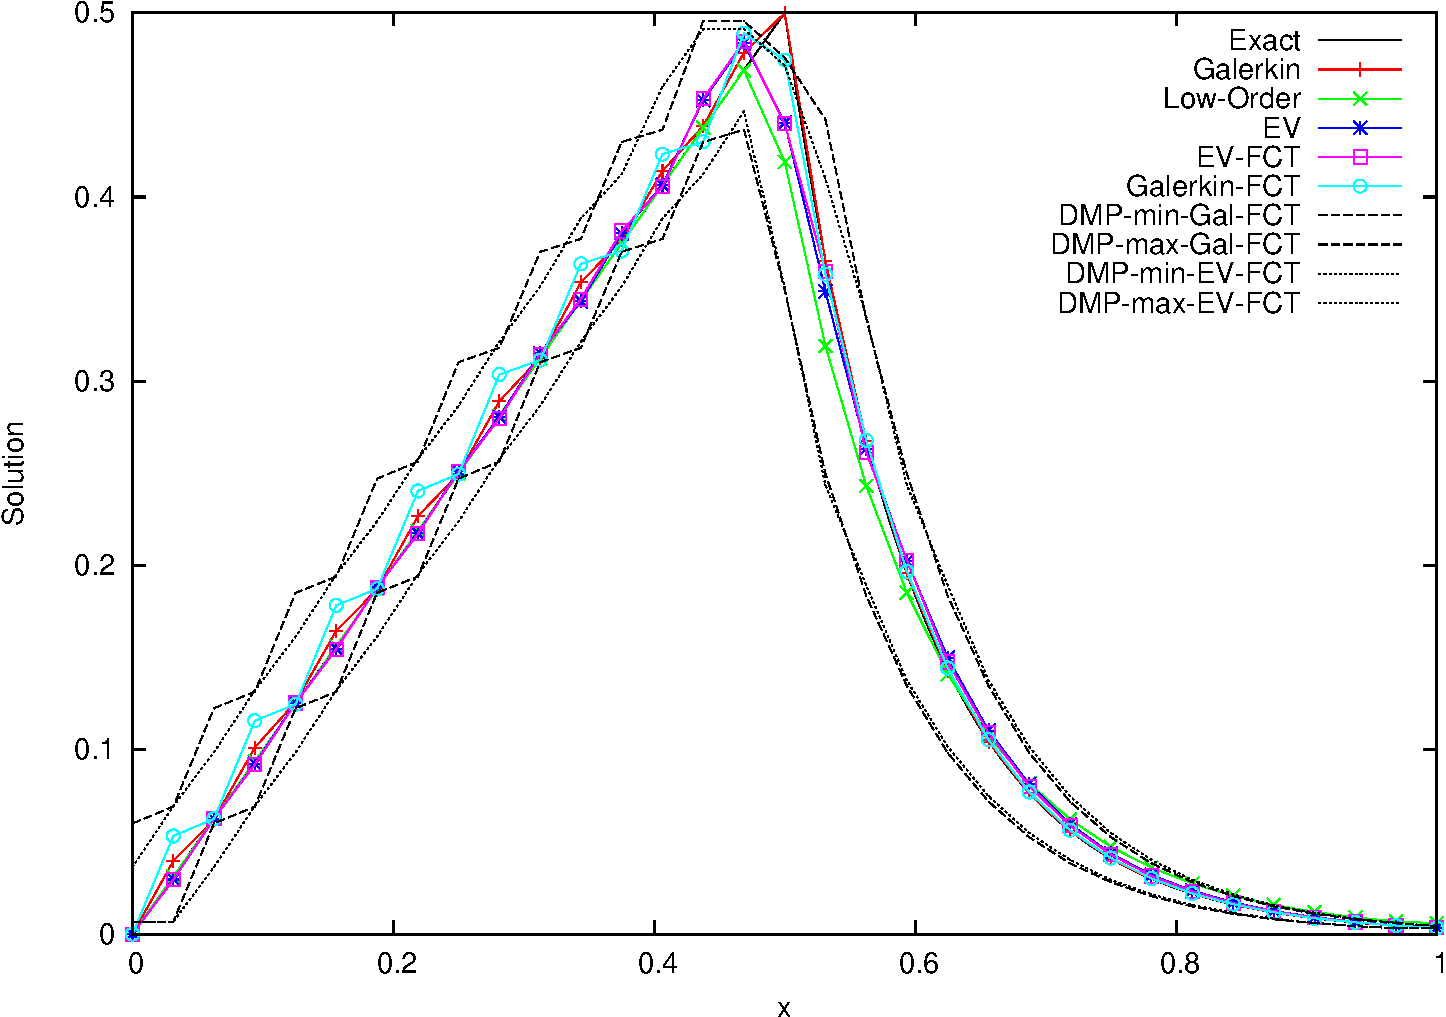
\includegraphics[width=\textwidth]
     {\contentdir/results/transport/source_void_to_absorber/coarse.pdf}
   \caption{Comparison of Solutions for the Source-Void-to-Absorber Problem
     Using SSPRK33 with 32 Cells}
   \label{fig:source_void_to_absorber}
\end{figure}
%-------------------------------------------------------------------------------
\begin{figure}[ht]
   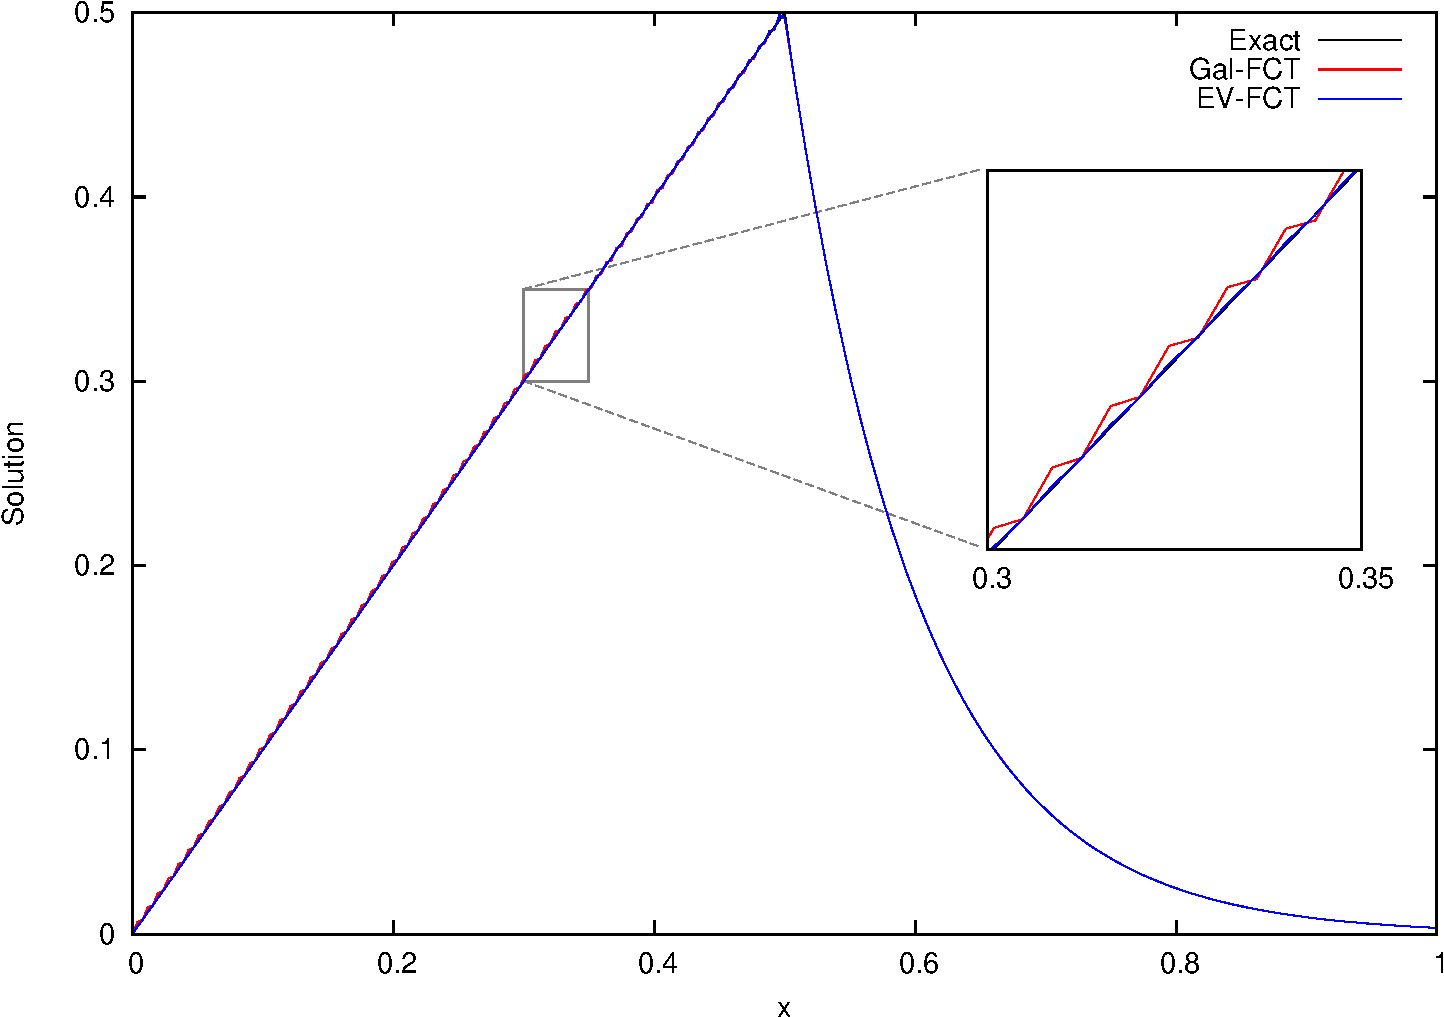
\includegraphics[width=\textwidth]
     {\contentdir/results/transport/source_void_to_absorber/fine.pdf}
   \caption{Comparison of Solutions for the Source-Void-to-Absorber Problem
     Using SSPRK33 with 256 Cells}
   \label{fig:source_void_to_absorber_fine}
\end{figure}
%-------------------------------------------------------------------------------

The steady-state results for this test problem revealed some significant
FCT issues regarding the antidiffusion from Dirichlet nodes.
When Dirichlet boundary conditions are strongly imposed, solution
bounds do not apply, and it becomes unclear how to limit antidiffusion
fluxes from these nodes. Consider symmetric limiters, i.e., those such that
$L\ij=L\ji$, such as Zalesak's limiter, for which
\begin{equation}
  L\ij = \left\{\begin{array}{c c}
    \min(L_i^+,L_j^-) & P\ij > 0\\
    \min(L_i^-,L_j^+) & P\ij < 0\\
  \end{array}\right. \eqp
\end{equation}
Suppose $i$ corresponds to a degree of freedom for which Dirichlet
boundary conditions are strongly imposed. The uncertainty
is the correct way to decide $L_i^+$ and $L_i^-$ since there
are no valid bounds from which to compute these values.
Figures \ref{fig:source_void_to_absorber_strong1} and 
\ref{fig:source_void_to_absorber_strong0} show the solutions obtained
using strongly imposed Dirichlet boundary conditions with these
values set to $L_i^+=L_i^-=1$ and $L_i^+=L_i^-=0$, respectively.
When $L_i^+=L_i^-=1$, the correction flux from the Dirichlet
DoF $i$, which is positive, has only the upper bound for $j$
to consider. The upper bound for $j$, which is inflated above the
analytical solution due to the source, does not restrict this
antidiffusion flux, and thus it is accepted fully to the unphysical
value. Due to the implicitness of the solution bounds, the lower solution
bound for $j$ is computed from this unphysical value and excludes the
possibility of antidiffusion back to the analytical solution. This
process continues with all of the other degrees of freedom.
When instead, $L_i^+=L_i^-=0$, the solution does not lie above
the analytical solution in the source region, but significant peak
clipping appears at the interface between the source and absorber
regions. It should be noted that there are combinations of limiting
coefficient values, each in the range $(0,1)$, that produce a more
accurate solution to this problem (without the peak clipping
and resulting inaccuracy in the absorber region); the problem is that Zalesak's
limiter (and in general, any practical limiter) is not optimal
in the sense that it maximizes the magnitude of antidiffusive flux.
One could in principle solve an optimization problem to select
limiting coefficients that maximize the antidiffusive flux, but this
is very expensive and thus not recommended for general use.

For weakly imposed Dirichlet boundary conditions, solution bounds
still apply, so limiting coefficients may be computed without special
consideration. However, one must now consider the possibility of
inaccurate boundary values.
Figures \ref{fig:source_void_to_absorber_weak} shows the steady-state 
solutions obtained using weakly imposed Dirichlet boundary conditions.
In this case, the antidiffusion flux from the boundary gets limited
(but not fully) due to the lower solution bound of the Dirichlet node.
Because some antidiffusion was accepted here, the peak reaches
a higher value than with the $L_i^+=L_i^-=0$ case.
Finally, Figure \ref{fig:source_void_to_absorber_penalty} shows
the steady-state solution obtained with weakly imposed Dirichlet
boundary conditions and a boundary penalty (see Section \ref{sec:transport_bc}).
The FCT solution looks very similar to the case without any penalty,
but the effect on the low-order and entropy viscosity solutions is
clear.

%-------------------------------------------------------------------------------
\begin{figure}[ht]
   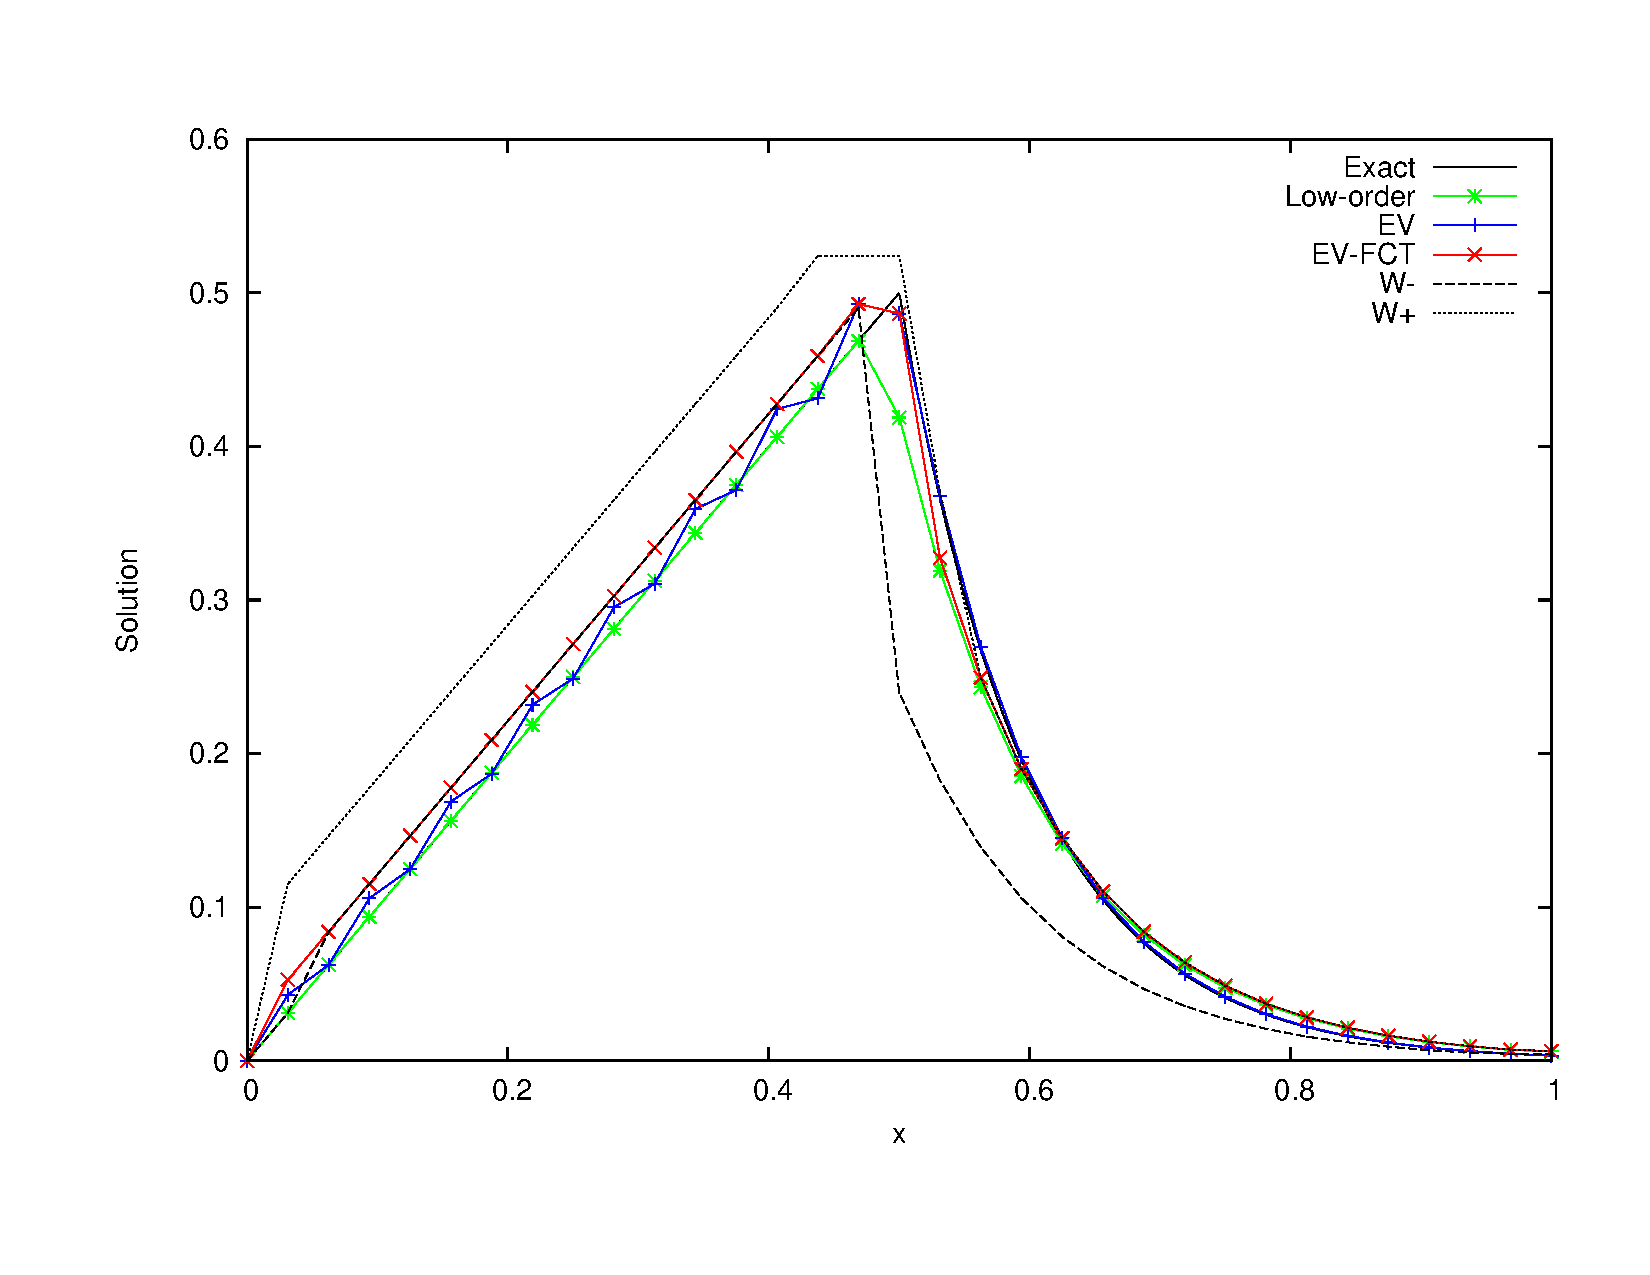
\includegraphics[width=\textwidth]
     {\contentdir/results/transport/source_void_to_absorber/images/strong1.pdf}
   \caption{Steady-State Solutions for the Source-Void-to-Absorber Problem
     with Strongly Imposed Dirichlet Boundary Conditions and $L^-=L^+=1$}
   \label{fig:source_void_to_absorber_strong1}
\end{figure}
%-------------------------------------------------------------------------------
%-------------------------------------------------------------------------------
\begin{figure}[ht]
   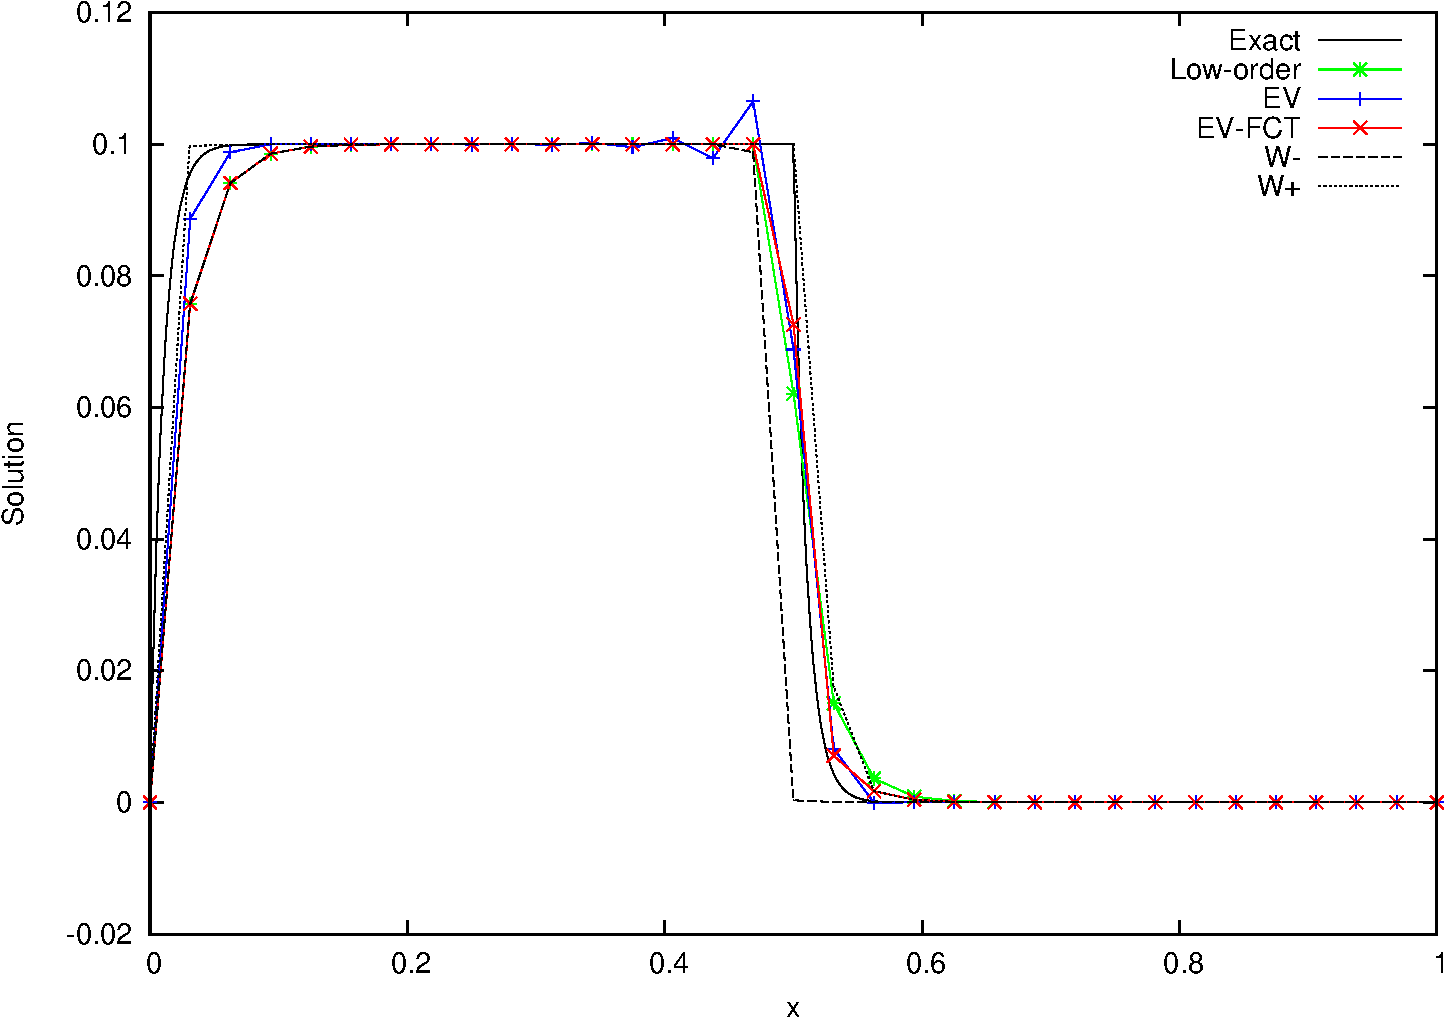
\includegraphics[width=\textwidth]
     {\contentdir/results/transport/source_void_to_absorber/images/strong0.pdf}
   \caption{Steady-State Solutions for the Source-Void-to-Absorber Problem
     with Strongly Imposed Dirichlet Boundary Conditions and $L^-=L^+=0$}
   \label{fig:source_void_to_absorber_strong0}
\end{figure}
%-------------------------------------------------------------------------------
%-------------------------------------------------------------------------------
\begin{figure}[ht]
   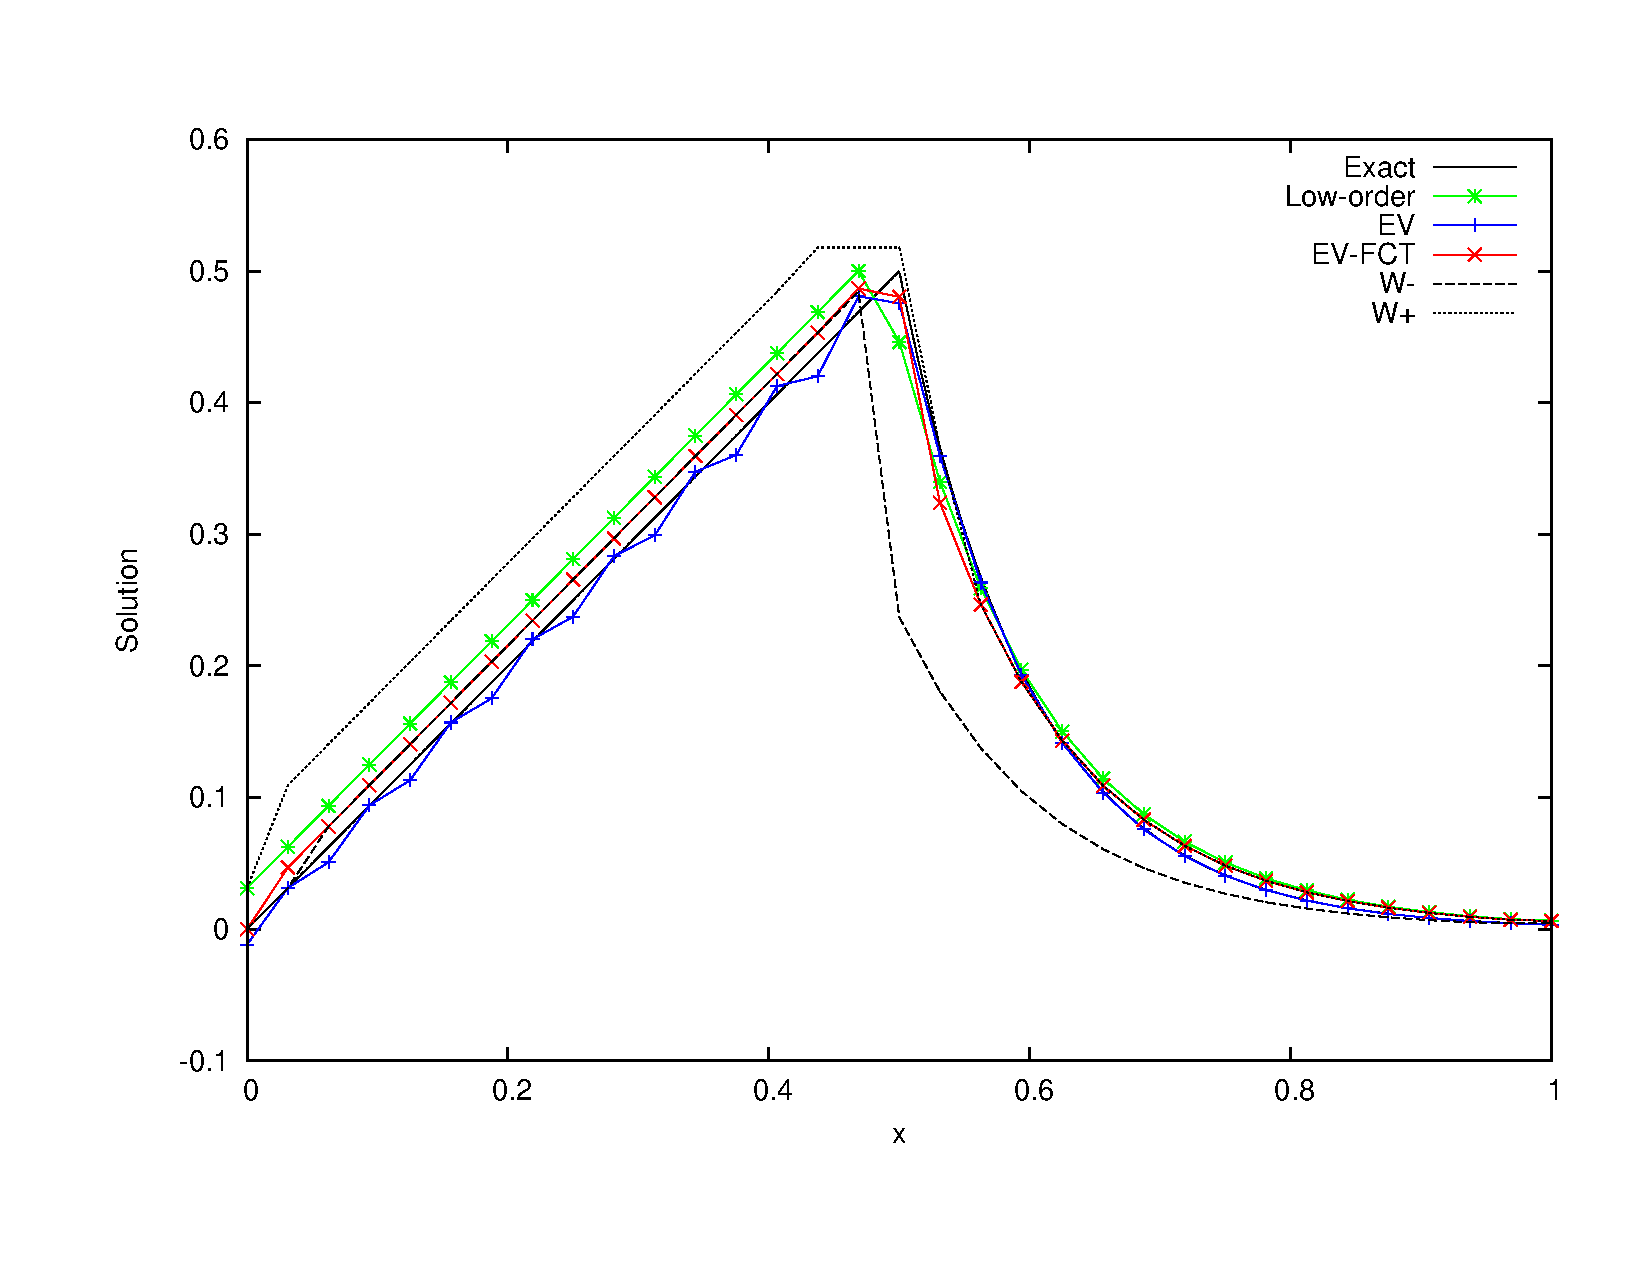
\includegraphics[width=\textwidth]
     {\contentdir/results/transport/source_void_to_absorber/images/weak.pdf}
   \caption{Steady-State Solutions for the Source-Void-to-Absorber Problem
     with Weakly Imposed Dirichlet Boundary Conditions}
   \label{fig:source_void_to_absorber_weak}
\end{figure}
%-------------------------------------------------------------------------------
%-------------------------------------------------------------------------------
\begin{figure}[ht]
   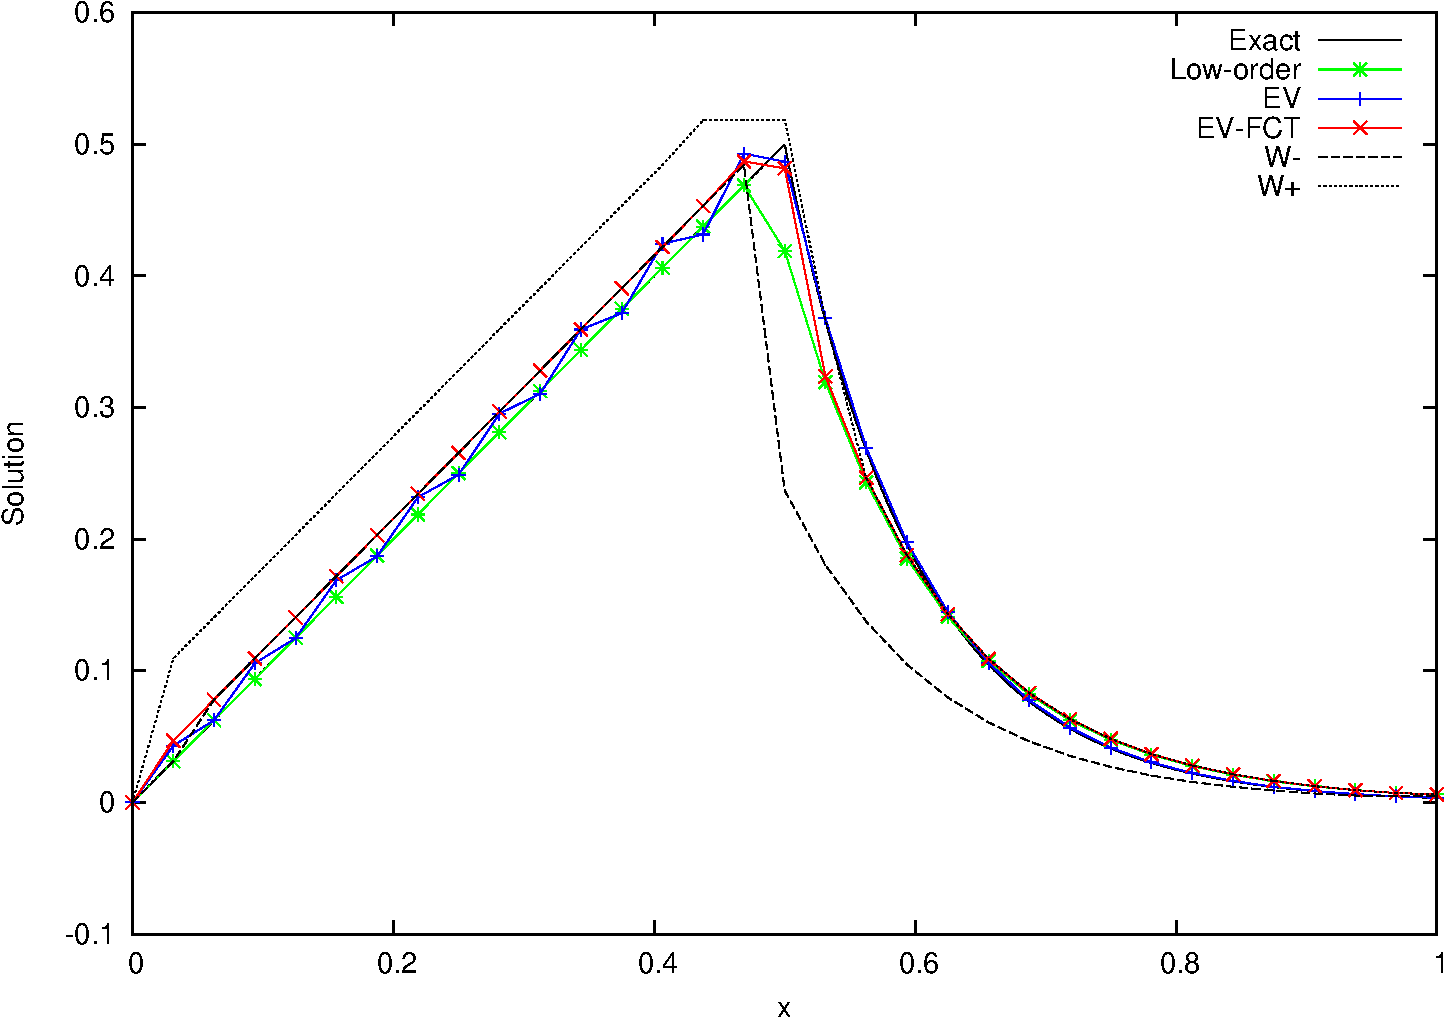
\includegraphics[width=\textwidth]
     {\contentdir/results/transport/source_void_to_absorber/images/weak_with_penalty.pdf}
   \caption{Steady-State Solutions for the Source-Void-to-Absorber Problem
     with Weakly Imposed Dirichlet Boundary Conditions and Boundary Penalty}
   \label{fig:source_void_to_absorber_penalty}
\end{figure}
%-------------------------------------------------------------------------------

Table \ref{tab:source_void_to_absorber_be_iterations_cells} shows the
results of a study of the number of EV and FCT iterations for
BE time discretization, required in
a transient with a constant CFL of 1 and varying mesh sizes. The
results in the table show a decrease in the number of EV iterations
per time step, and a relatively constant number of FCT iterations per
time step.

%-------------------------------------------------------------------------------
\begin{center}
\begin{table}[ht]
\caption{Nonlinear Iterations vs. Number of Cells for the
  Source-Void-to-Absorber Test Problem Using Implicit Euler Time Discretization
  with CFL = 1}
\label{tab:source_void_to_absorber_be_iterations_cells}
\begin{tabular}{c c c c c}\toprule
$N_{cell}$ & \multicolumn{2}{c}{\emph{EV}} & \multicolumn{2}{c}{\emph{FCT}}\\
           & \emph{Total} & \emph{Avg.}    &  \emph{Total} & \emph{Avg.}\\\midrule
  8 &  661 & 24.48 &   244 &  9.04\\
 16 &  807 & 19.21 &   655 & 15.60\\
 32 &  844 & 11.25 &  1194 & 15.92\\
 64 & 1204 &  8.72 &  2024 & 14.67\\
128 & 1752 &  6.59 &  3675 & 13.82\\
256 & 2713 &  5.20 &  6673 & 12.78\\
512 & 4284 &  4.14 & 12098 & 11.69\\
\bottomrule\end{tabular}
\end{table}
\end{center}
%-------------------------------------------------------------------------------

Table \ref{tab:source_void_to_absorber_be_iterations_cfl} shows
the results of a study of nonlinear iterations vs. CFL number for
implicit Euler time discretization and 128 cells. The general
trend shows that entropy viscosity iterations per time step gradually increase
with increasing CFL, while FCT iterations per time step increases
much more quickly. Even more problematic is that the EV-FCT solution
error jumps very quickly from CFLs $\nu=5$ to $\nu=10$.

%-------------------------------------------------------------------------------
\begin{table}[htb]
\caption{Nonlinear Iterations vs. CFL Number for the
 Source-Void-to-Absorber Test Problem Using Implicit Euler Time Discretization
 with 128 Cells}
\label{tab:source_void_to_absorber_be_iterations_cfl}
\centering
\begin{tabular}{c c c c c c c }\toprule
 & & \multicolumn{2}{c}{\emph{EV}}
  & \multicolumn{2}{c}{\emph{FCT}} &\\
\emph{CFL} & $N_{step}$ & \emph{Total} & \emph{Avg.}
  & \emph{Total} & \emph{Avg.} & $L^2$ \emph{err.}\\\midrule
0.1 & 2661 & 15006 &  5.64 & 14036 &   5.27 & $3.013\times10^{-3}$\\
0.5 &  533 &  3445 &  6.46 &  5000 &   9.38 & $3.033\times10^{-3}$\\
1.0 &  266 &  1752 &  6.59 &  3675 &  13.82 & $3.023\times10^{-3}$\\
5.0 &   54 &   471 &  8.72 & 12208 & 226.07 & $2.979\times10^{-3}$\\
10.0 &  27 &   232 &  8.59 &  6126 & 226.89 & $3.325\times10^{-3}$\\
20.0 &  14 &   133 &  9.50 &  3713 & 265.21 & $3.727\times10^{-3}$\\
50.0 &   6 &    62 & 10.33 &  2077 & 346.17 & $7.191\times10^{-3}$\\
\bottomrule\end{tabular}
\end{table}
%-------------------------------------------------------------------------------

\clearpage

In this section, results are presented for the
source-void-to-absorber test problem. This is a 1-D test problem
with zero incoming flux incident on the left boundary,
a constant source in a void in the left half of the
domain, and an absorber with no source in the right half of the
domain. The test problem description is given by Table
\ref{tab:source_void_to_absorber}.

%-------------------------------------------------------------------------------
\begin{table}[htb]\caption{Source-Void-to-Absorber Test Problem Summary}
\label{tab:source_void_to_absorber}
\centering
\begin{tabular}{l l}\toprule
\emph{Parameter} & \emph{Value}\\\midrule
Domain & $\domain = (0,1)$\\
Initial Conditions & $u_0(x)=0$\\
Boundary Conditions & $u(0,t)=0 \eqc \quad t>0$\\
Direction & $\di = \mathbf{e}_x$\\
Cross Section & $\sigma(x)=\left\{\begin{array}{c l}
   0,  & x < \frac{1}{2}\\
   10, & \mbox{otherwise}\end{array}\right.$\\
Source & $q(\x,t)=\left\{\begin{array}{c l}
   1,  & x < \frac{1}{2}\\
   0,  & \mbox{otherwise}\end{array}\right.$\\
Speed & $\speed=1$\\
Exact Solution & $u(x,t)=\left\{\begin{array}{l l}
   \scalarsolution_{\text{ss}}(x), & x-t<0\\
   0, & \mbox{otherwise}
   \end{array}\right.$ \\
   & $\scalarsolution_{\text{ss}}(x) =
       \left\{\begin{array}{l l}
          e^{-10(x-\frac{1}{2})}, & x\ge\frac{1}{2}\\
          1,                      & \mbox{otherwise}
       \end{array}\right.$\\
\bottomrule\end{tabular}
\end{table}
%-------------------------------------------------------------------------------

Figure \ref{fig:source_void_to_absorber}
shows the results for this problem using SSPRK time discretization,
a CFL of 0.5, and 32 cells.
Entropy residual and jump coefficients $\entropyresidualcoef$ and
$\entropyjumpcoef$ are both 1.
Table \ref{tab:source_void_to_absorber_run_parameters} summarizes the
run parameters to generate the results in this section.
Figure \ref{fig:source_void_to_absorber_fine} shows results
for a finer mesh (256 cells) that illustrates the shortcomings of Galerkin-FCT
vs. EV-FCT: Galerkin-FCT does not necessarily converge to the
entropy solution.

%-------------------------------------------------------------------------------
\begin{table}[ht]\caption{Source-Void-to-Absorber Test Problem Run Parameters}
\label{tab:source_void_to_absorber_run_parameters}
\centering
\begin{tabular}{l l}\toprule
\emph{Parameter} & \emph{Value}\\\midrule
Number of Cells & $N_{cell} = 32, 256$\\
End Time & $t = 1$\\
CFL Number & $\nu = 0.5$\\\midrule
Entropy Function & $\entropy(u) = \frac{1}{2}u^2$\\
Entropy Residual Coefficient & $\entropyresidualcoef = 1$\\
Entropy Jump Coefficient & $\entropyjumpcoef = 1$\\
\bottomrule\end{tabular}
\end{table}
%-------------------------------------------------------------------------------
\begin{figure}[ht]
   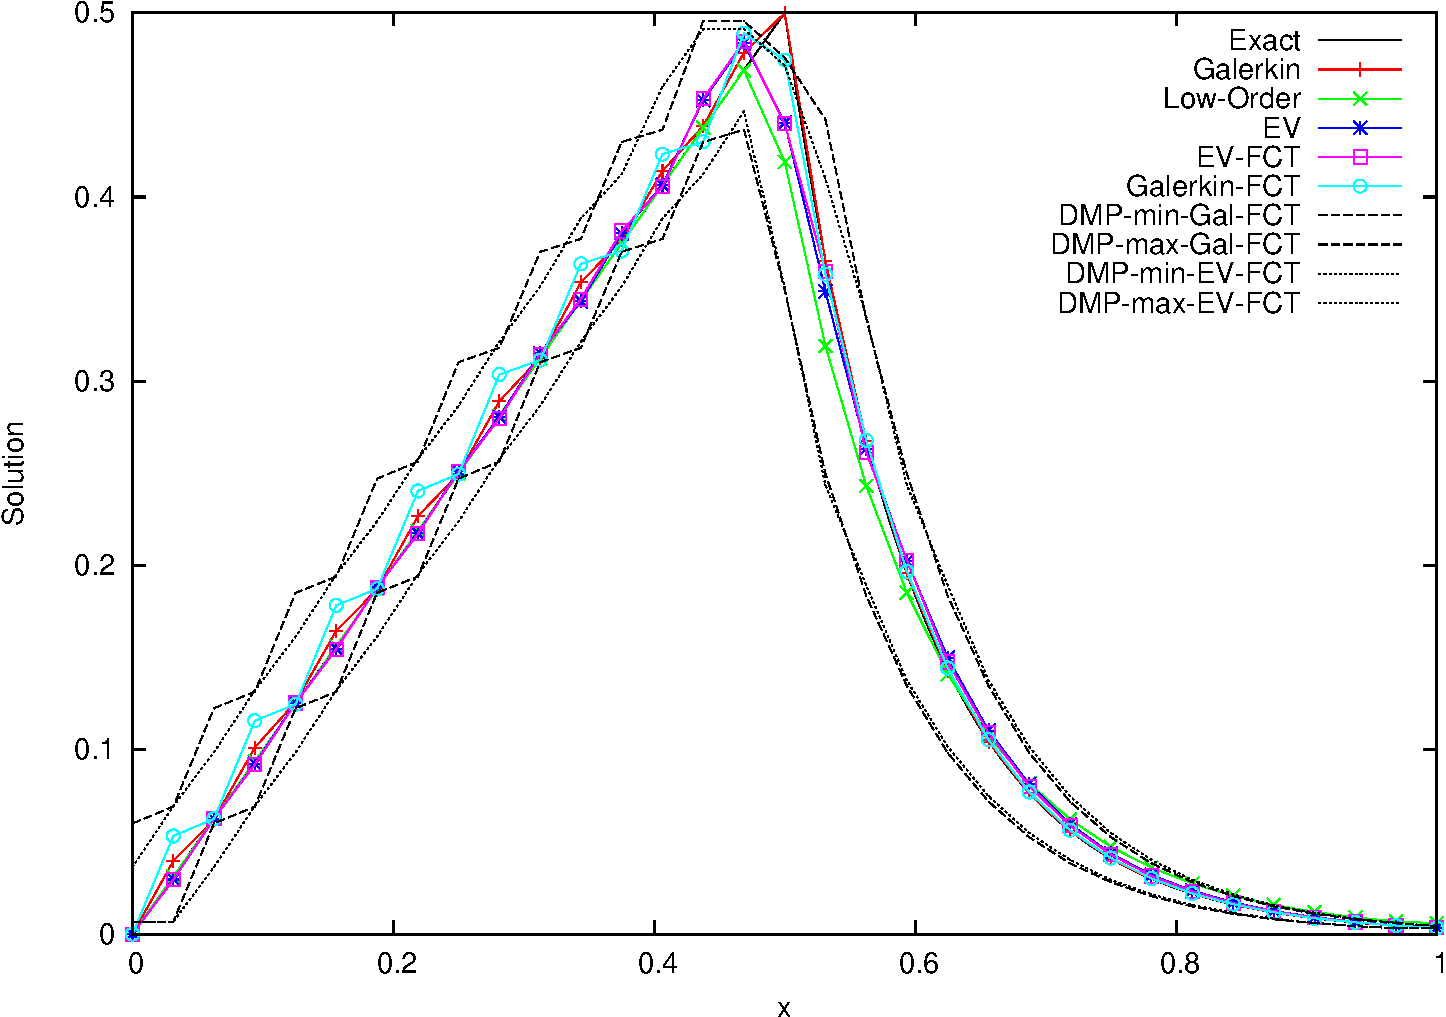
\includegraphics[width=\textwidth]
     {\contentdir/results/transport/source_void_to_absorber/coarse.pdf}
   \caption{Comparison of Solutions for the Source-Void-to-Absorber Problem
     Using SSPRK33 with 32 Cells}
   \label{fig:source_void_to_absorber}
\end{figure}
%-------------------------------------------------------------------------------
\begin{figure}[ht]
   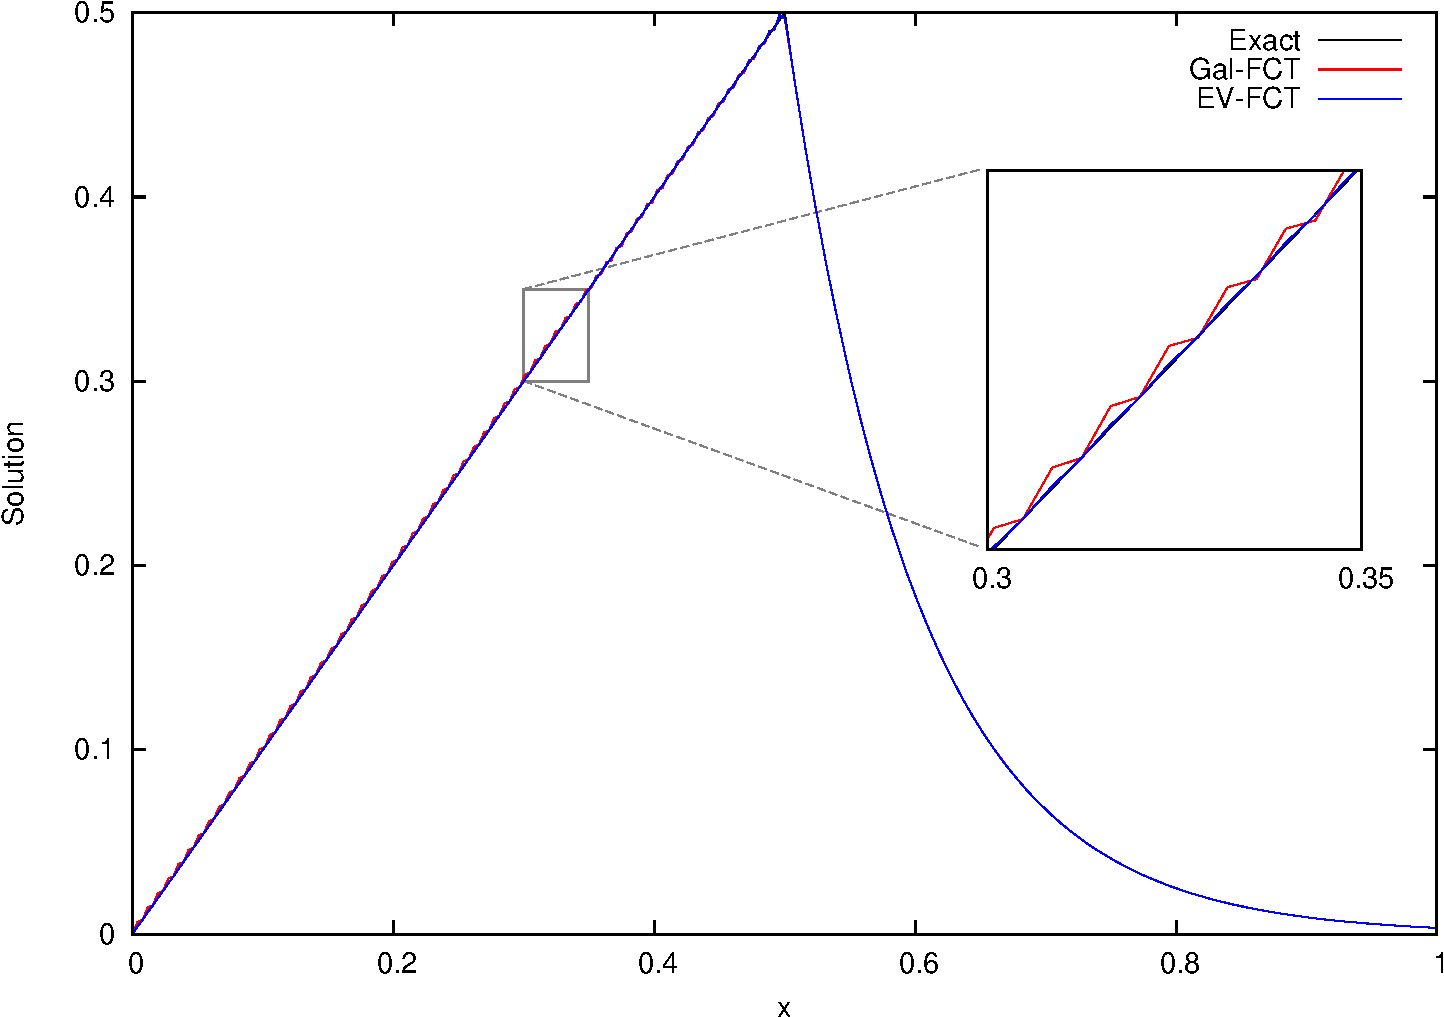
\includegraphics[width=\textwidth]
     {\contentdir/results/transport/source_void_to_absorber/fine.pdf}
   \caption{Comparison of Solutions for the Source-Void-to-Absorber Problem
     Using SSPRK33 with 256 Cells}
   \label{fig:source_void_to_absorber_fine}
\end{figure}
%-------------------------------------------------------------------------------

The steady-state results for this test problem revealed some significant
FCT issues regarding the antidiffusion from Dirichlet nodes.
When Dirichlet boundary conditions are strongly imposed, solution
bounds do not apply, and it becomes unclear how to limit antidiffusion
fluxes from these nodes. Consider symmetric limiters, i.e., those such that
$L\ij=L\ji$, such as Zalesak's limiter, for which
\begin{equation}
  L\ij = \left\{\begin{array}{c c}
    \min(L_i^+,L_j^-) & P\ij > 0\\
    \min(L_i^-,L_j^+) & P\ij < 0\\
  \end{array}\right. \eqp
\end{equation}
Suppose $i$ corresponds to a degree of freedom for which Dirichlet
boundary conditions are strongly imposed. The uncertainty
is the correct way to decide $L_i^+$ and $L_i^-$ since there
are no valid bounds from which to compute these values.
Figures \ref{fig:source_void_to_absorber_strong1} and 
\ref{fig:source_void_to_absorber_strong0} show the solutions obtained
using strongly imposed Dirichlet boundary conditions with these
values set to $L_i^+=L_i^-=1$ and $L_i^+=L_i^-=0$, respectively.
When $L_i^+=L_i^-=1$, the correction flux from the Dirichlet
DoF $i$, which is positive, has only the upper bound for $j$
to consider. The upper bound for $j$, which is inflated above the
analytical solution due to the source, does not restrict this
antidiffusion flux, and thus it is accepted fully to the unphysical
value. Due to the implicitness of the solution bounds, the lower solution
bound for $j$ is computed from this unphysical value and excludes the
possibility of antidiffusion back to the analytical solution. This
process continues with all of the other degrees of freedom.
When instead, $L_i^+=L_i^-=0$, the solution does not lie above
the analytical solution in the source region, but significant peak
clipping appears at the interface between the source and absorber
regions. It should be noted that there are combinations of limiting
coefficient values, each in the range $(0,1)$, that produce a more
accurate solution to this problem (without the peak clipping
and resulting inaccuracy in the absorber region); the problem is that Zalesak's
limiter (and in general, any practical limiter) is not optimal
in the sense that it maximizes the magnitude of antidiffusive flux.
One could in principle solve an optimization problem to select
limiting coefficients that maximize the antidiffusive flux, but this
is very expensive and thus not recommended for general use.

For weakly imposed Dirichlet boundary conditions, solution bounds
still apply, so limiting coefficients may be computed without special
consideration. However, one must now consider the possibility of
inaccurate boundary values.
Figures \ref{fig:source_void_to_absorber_weak} shows the steady-state 
solutions obtained using weakly imposed Dirichlet boundary conditions.
In this case, the antidiffusion flux from the boundary gets limited
(but not fully) due to the lower solution bound of the Dirichlet node.
Because some antidiffusion was accepted here, the peak reaches
a higher value than with the $L_i^+=L_i^-=0$ case.
Finally, Figure \ref{fig:source_void_to_absorber_penalty} shows
the steady-state solution obtained with weakly imposed Dirichlet
boundary conditions and a boundary penalty (see Section \ref{sec:transport_bc}).
The FCT solution looks very similar to the case without any penalty,
but the effect on the low-order and entropy viscosity solutions is
clear.

%-------------------------------------------------------------------------------
\begin{figure}[ht]
   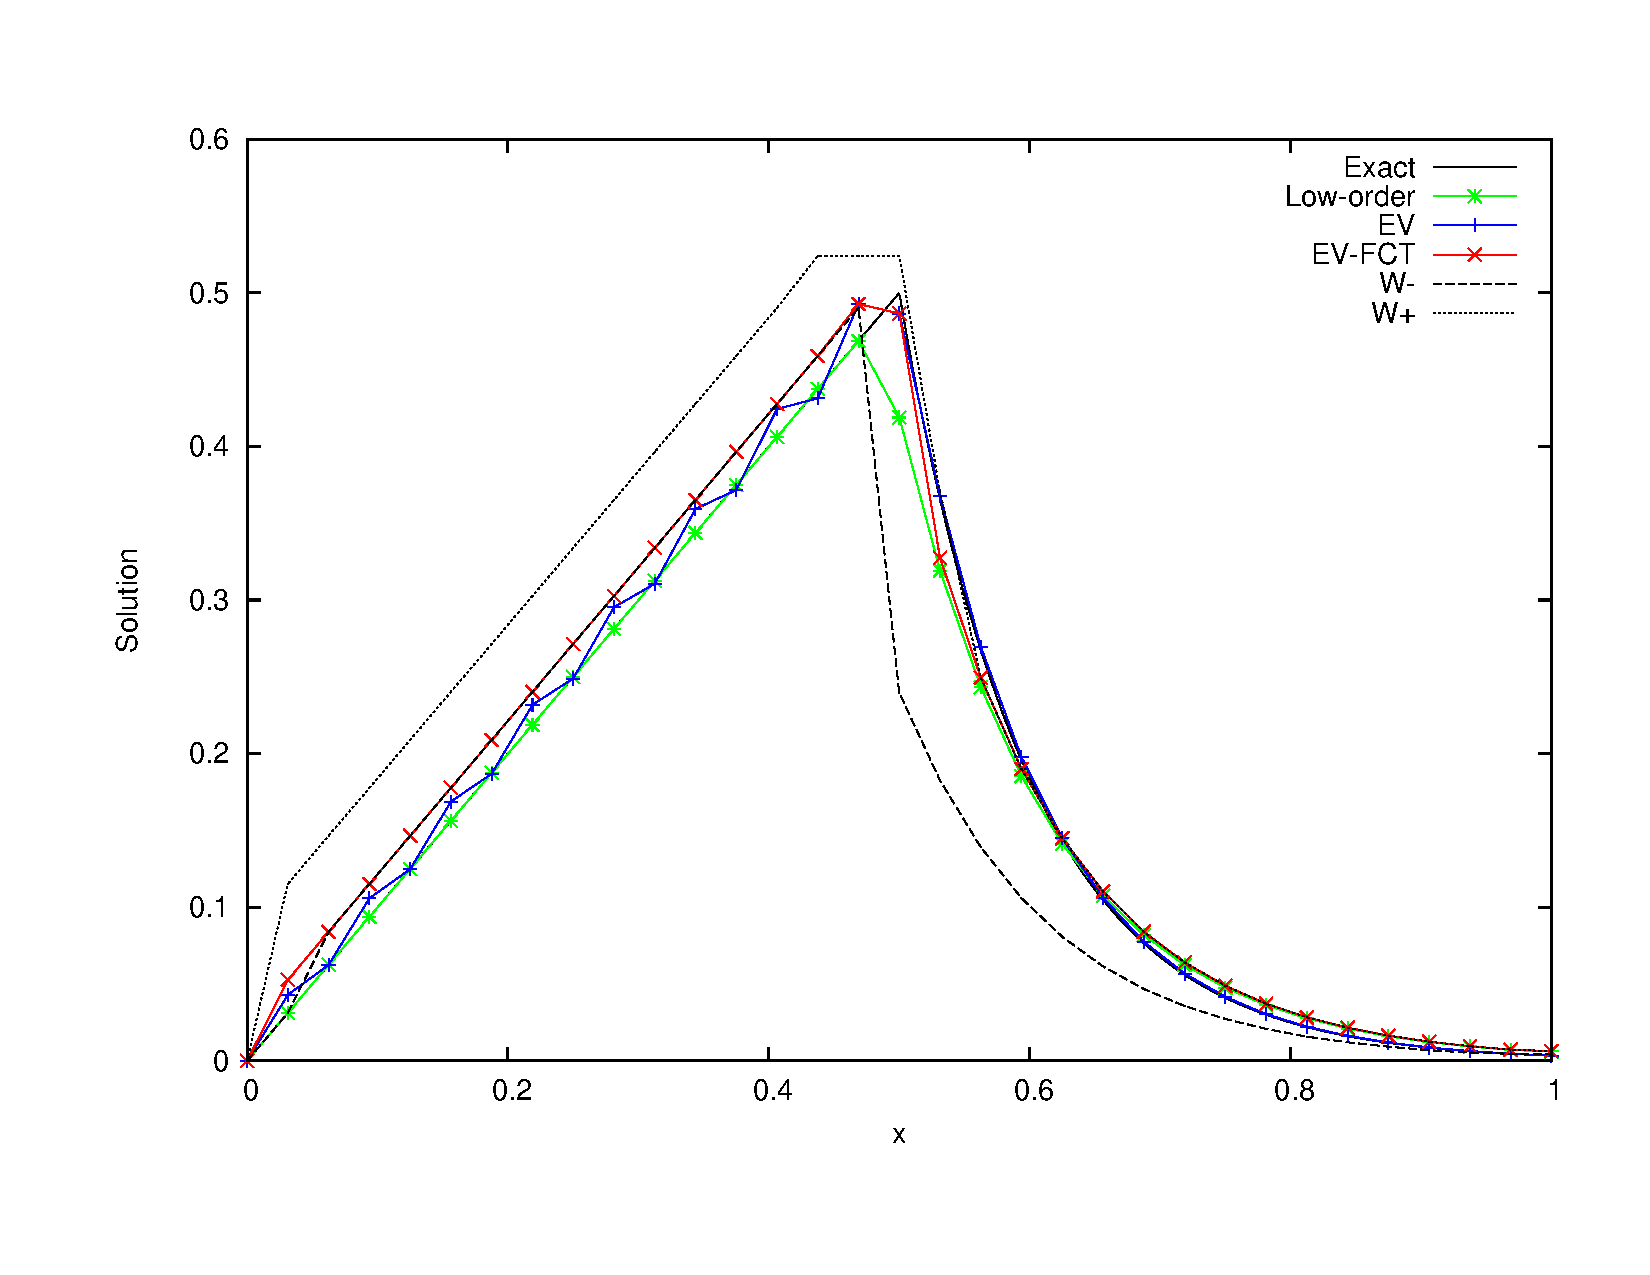
\includegraphics[width=\textwidth]
     {\contentdir/results/transport/source_void_to_absorber/images/strong1.pdf}
   \caption{Steady-State Solutions for the Source-Void-to-Absorber Problem
     with Strongly Imposed Dirichlet Boundary Conditions and $L^-=L^+=1$}
   \label{fig:source_void_to_absorber_strong1}
\end{figure}
%-------------------------------------------------------------------------------
%-------------------------------------------------------------------------------
\begin{figure}[ht]
   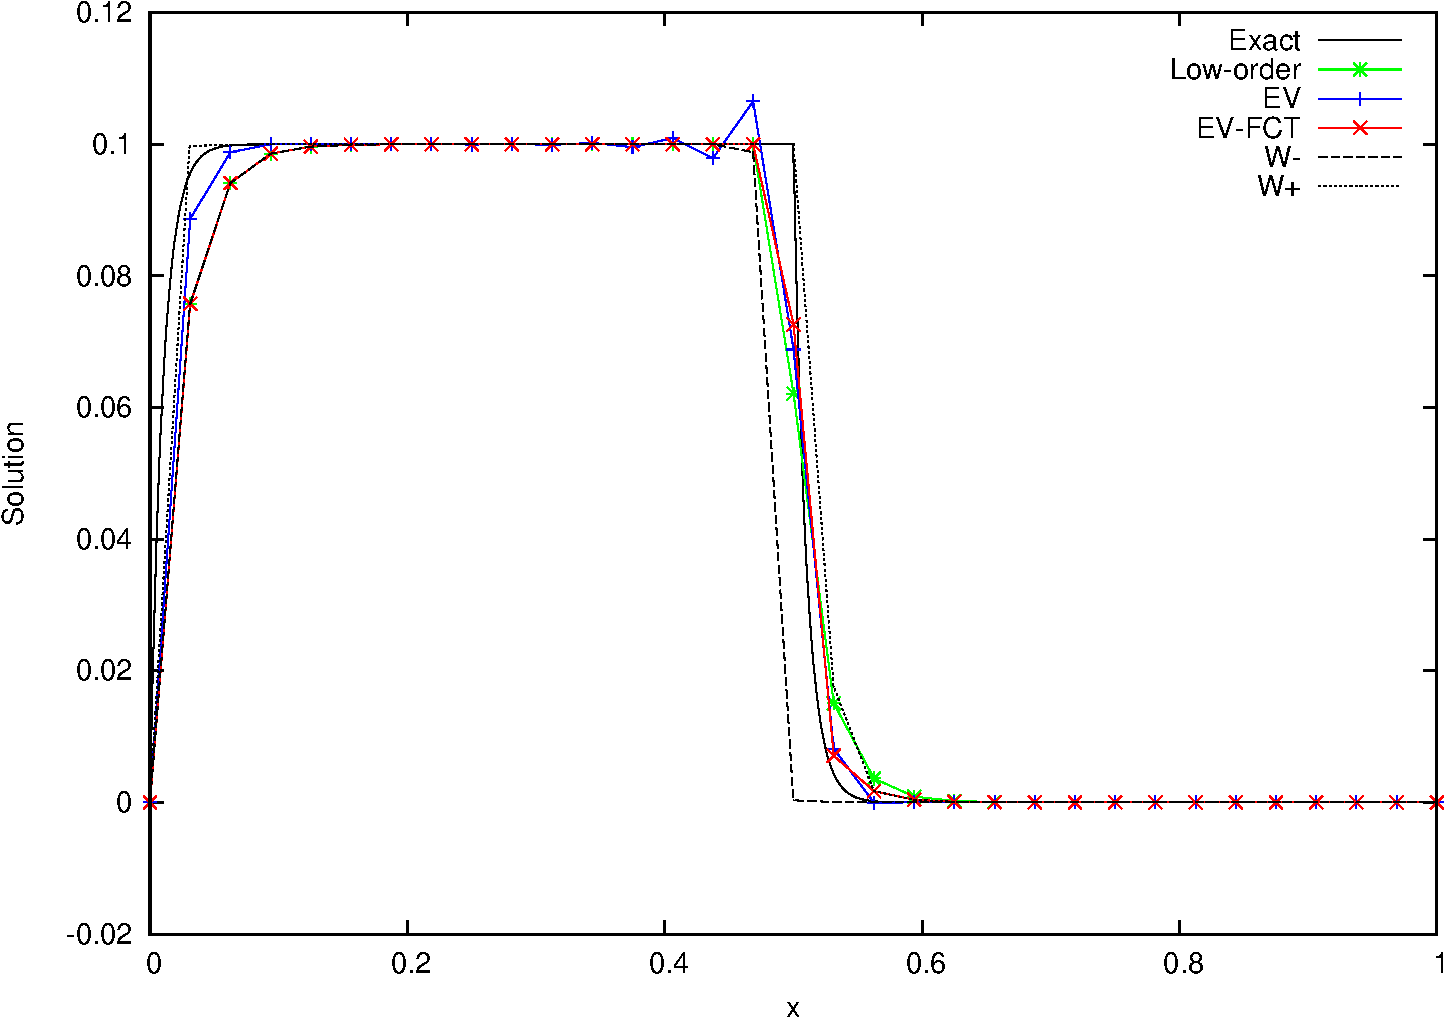
\includegraphics[width=\textwidth]
     {\contentdir/results/transport/source_void_to_absorber/images/strong0.pdf}
   \caption{Steady-State Solutions for the Source-Void-to-Absorber Problem
     with Strongly Imposed Dirichlet Boundary Conditions and $L^-=L^+=0$}
   \label{fig:source_void_to_absorber_strong0}
\end{figure}
%-------------------------------------------------------------------------------
%-------------------------------------------------------------------------------
\begin{figure}[ht]
   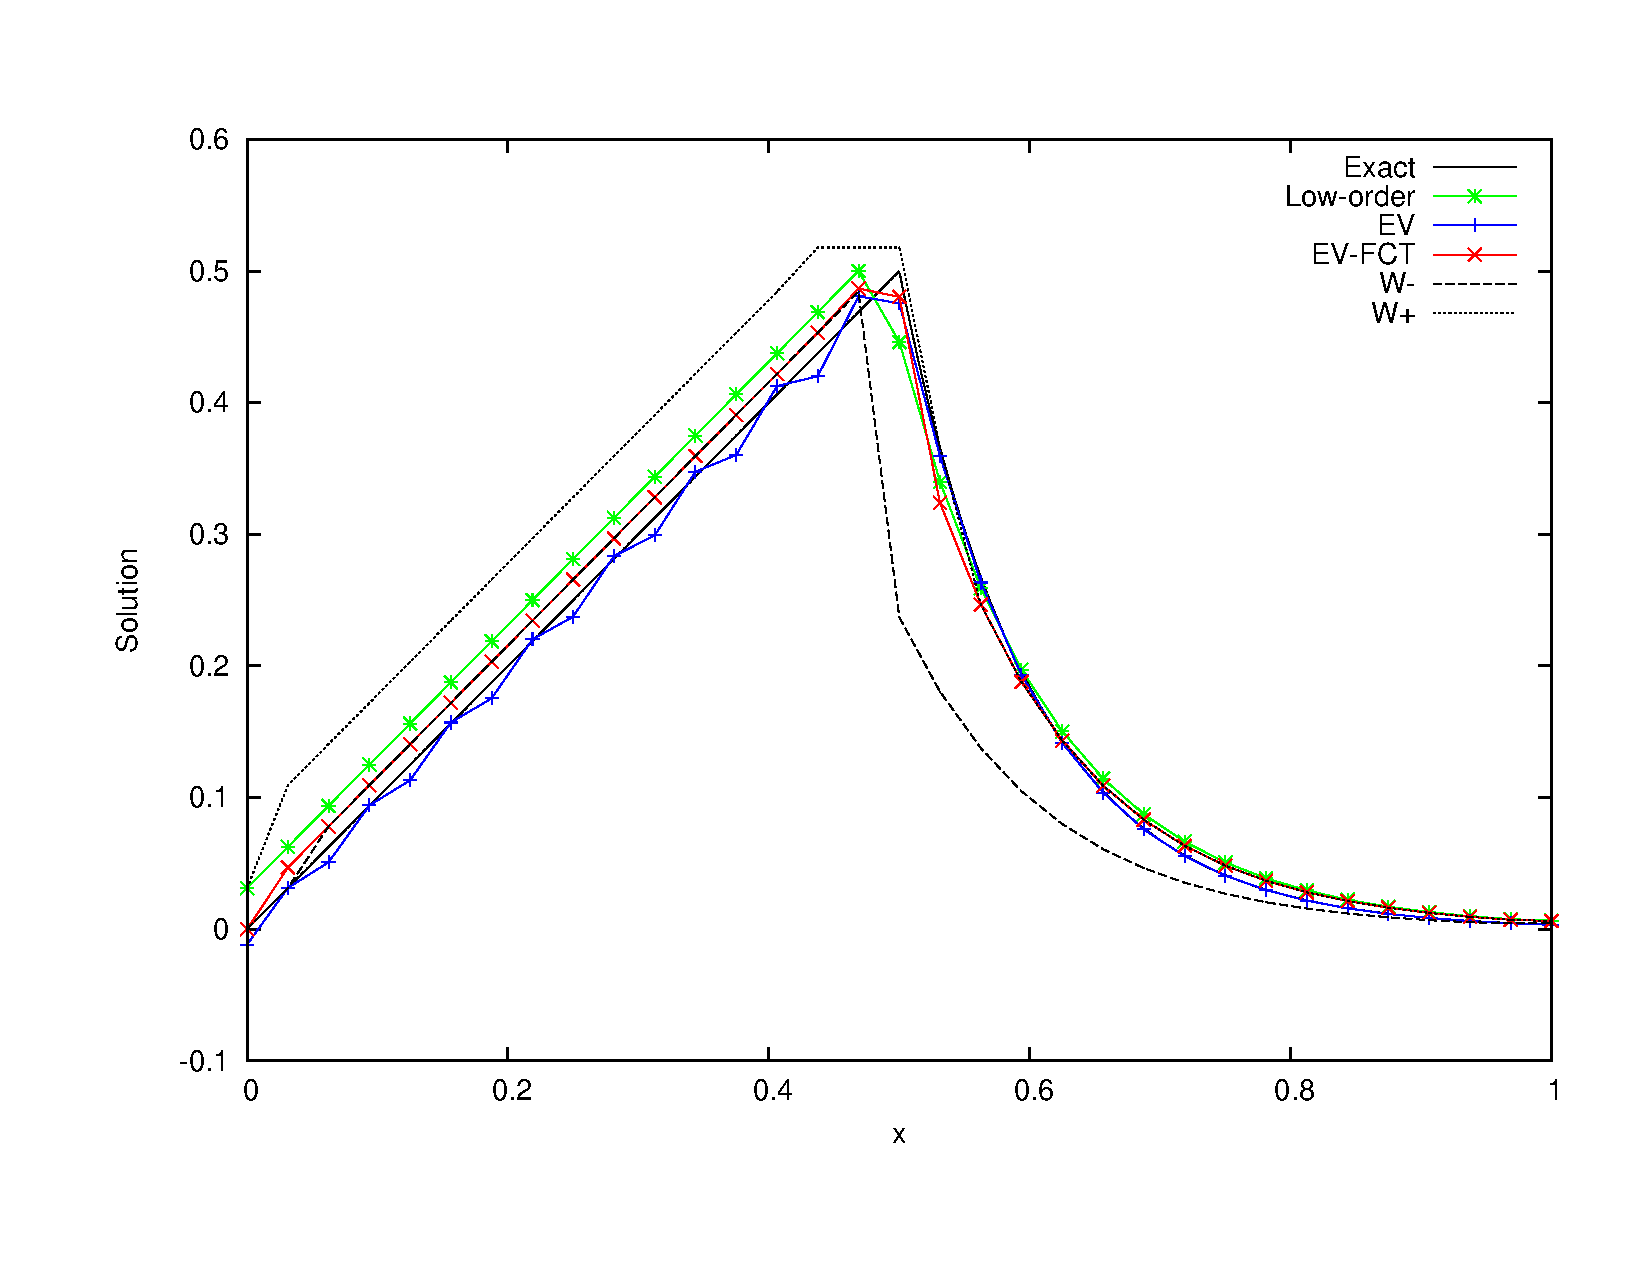
\includegraphics[width=\textwidth]
     {\contentdir/results/transport/source_void_to_absorber/images/weak.pdf}
   \caption{Steady-State Solutions for the Source-Void-to-Absorber Problem
     with Weakly Imposed Dirichlet Boundary Conditions}
   \label{fig:source_void_to_absorber_weak}
\end{figure}
%-------------------------------------------------------------------------------
%-------------------------------------------------------------------------------
\begin{figure}[ht]
   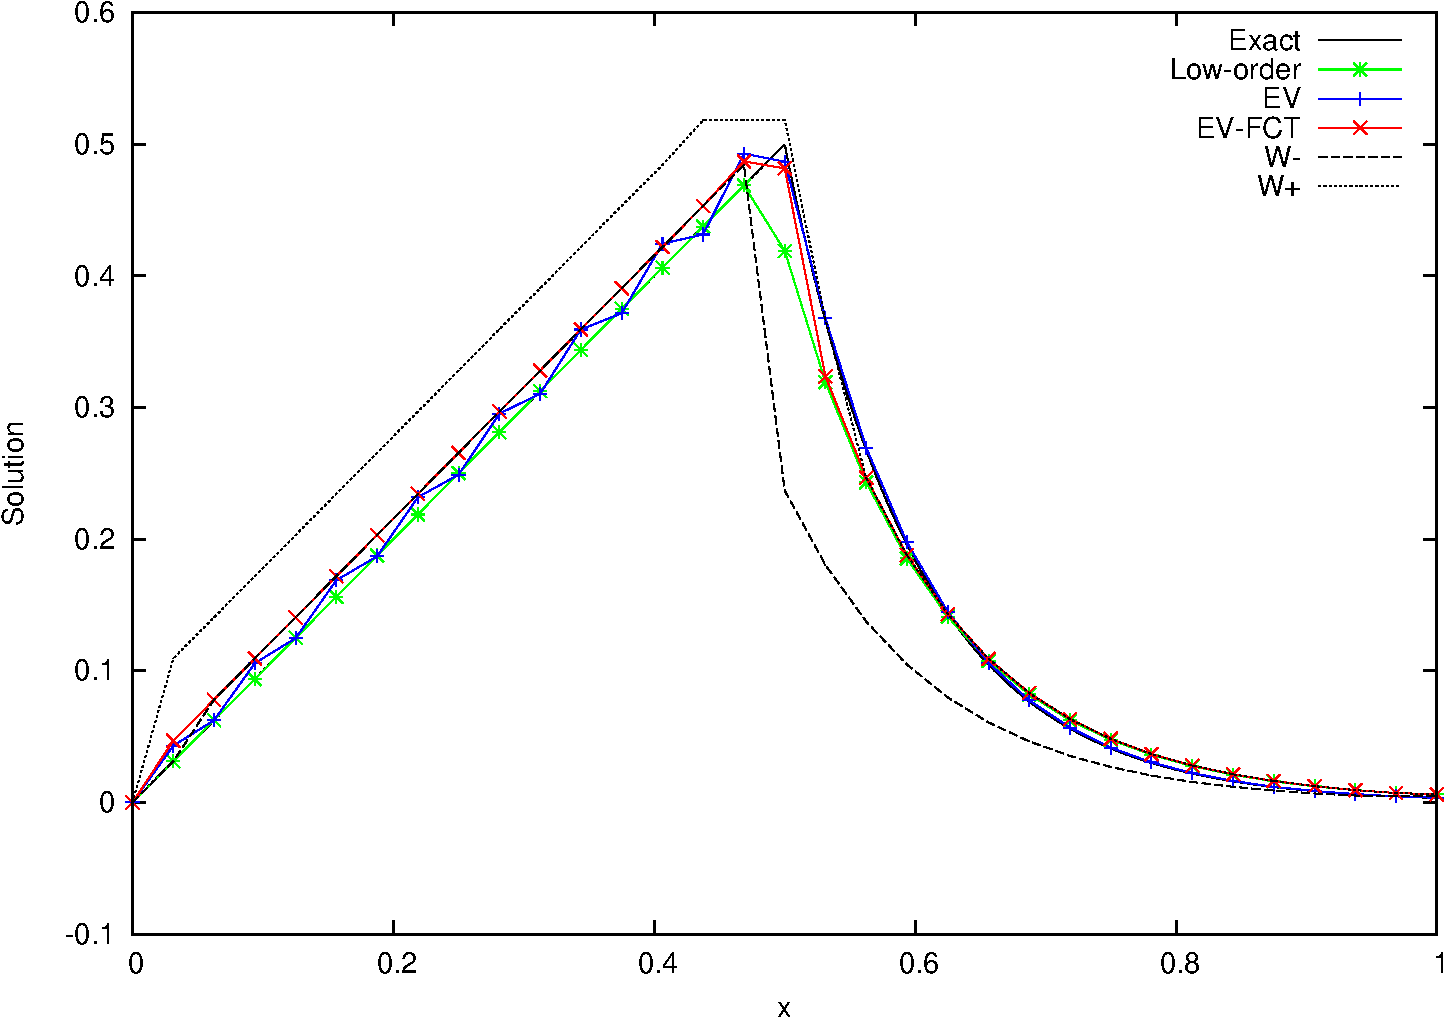
\includegraphics[width=\textwidth]
     {\contentdir/results/transport/source_void_to_absorber/images/weak_with_penalty.pdf}
   \caption{Steady-State Solutions for the Source-Void-to-Absorber Problem
     with Weakly Imposed Dirichlet Boundary Conditions and Boundary Penalty}
   \label{fig:source_void_to_absorber_penalty}
\end{figure}
%-------------------------------------------------------------------------------

Table \ref{tab:source_void_to_absorber_be_iterations_cells} shows the
results of a study of the number of EV and FCT iterations for
BE time discretization, required in
a transient with a constant CFL of 1 and varying mesh sizes. The
results in the table show a decrease in the number of EV iterations
per time step, and a relatively constant number of FCT iterations per
time step.

%-------------------------------------------------------------------------------
\begin{center}
\begin{table}[ht]
\caption{Nonlinear Iterations vs. Number of Cells for the
  Source-Void-to-Absorber Test Problem Using Implicit Euler Time Discretization
  with CFL = 1}
\label{tab:source_void_to_absorber_be_iterations_cells}
\begin{tabular}{c c c c c}\toprule
$N_{cell}$ & \multicolumn{2}{c}{\emph{EV}} & \multicolumn{2}{c}{\emph{FCT}}\\
           & \emph{Total} & \emph{Avg.}    &  \emph{Total} & \emph{Avg.}\\\midrule
  8 &  661 & 24.48 &   244 &  9.04\\
 16 &  807 & 19.21 &   655 & 15.60\\
 32 &  844 & 11.25 &  1194 & 15.92\\
 64 & 1204 &  8.72 &  2024 & 14.67\\
128 & 1752 &  6.59 &  3675 & 13.82\\
256 & 2713 &  5.20 &  6673 & 12.78\\
512 & 4284 &  4.14 & 12098 & 11.69\\
\bottomrule\end{tabular}
\end{table}
\end{center}
%-------------------------------------------------------------------------------

Table \ref{tab:source_void_to_absorber_be_iterations_cfl} shows
the results of a study of nonlinear iterations vs. CFL number for
implicit Euler time discretization and 128 cells. The general
trend shows that entropy viscosity iterations per time step gradually increase
with increasing CFL, while FCT iterations per time step increases
much more quickly. Even more problematic is that the EV-FCT solution
error jumps very quickly from CFLs $\nu=5$ to $\nu=10$.

%-------------------------------------------------------------------------------
\begin{table}[htb]
\caption{Nonlinear Iterations vs. CFL Number for the
 Source-Void-to-Absorber Test Problem Using Implicit Euler Time Discretization
 with 128 Cells}
\label{tab:source_void_to_absorber_be_iterations_cfl}
\centering
\begin{tabular}{c c c c c c c }\toprule
 & & \multicolumn{2}{c}{\emph{EV}}
  & \multicolumn{2}{c}{\emph{FCT}} &\\
\emph{CFL} & $N_{step}$ & \emph{Total} & \emph{Avg.}
  & \emph{Total} & \emph{Avg.} & $L^2$ \emph{err.}\\\midrule
0.1 & 2661 & 15006 &  5.64 & 14036 &   5.27 & $3.013\times10^{-3}$\\
0.5 &  533 &  3445 &  6.46 &  5000 &   9.38 & $3.033\times10^{-3}$\\
1.0 &  266 &  1752 &  6.59 &  3675 &  13.82 & $3.023\times10^{-3}$\\
5.0 &   54 &   471 &  8.72 & 12208 & 226.07 & $2.979\times10^{-3}$\\
10.0 &  27 &   232 &  8.59 &  6126 & 226.89 & $3.325\times10^{-3}$\\
20.0 &  14 &   133 &  9.50 &  3713 & 265.21 & $3.727\times10^{-3}$\\
50.0 &   6 &    62 & 10.33 &  2077 & 346.17 & $7.191\times10^{-3}$\\
\bottomrule\end{tabular}
\end{table}
%-------------------------------------------------------------------------------

\clearpage

\end{document}

  }
  \block{Conclusions}{
    The FCT scheme described in this paper is second-order accurate in space,
converges to the entropy solution, and preserves non-negativity.
Spurious oscillations are mitigated but are not guaranteed to be
eliminated, as smaller magnitude oscillations may exist within the imposed
solution bounds.

% Local solution bounds imposed in the FCT algorithm were derived using the method
% of characteristics and integral transport equation.
% Two sets of solution
% bounds were considered, one considering only values along the upstream
% line segment traversed in a time step, and the other considering a spherical
% neighborhood that encompasses this line segment. The former set of solution
% bounds is much tighter, which has the advantage that there is a smaller range
% of limiting coefficient values that can be used, but has the disadvantage that
% there is less room for antidiffusion.

The traditional FCT phenomenon known as ``stair-stepping'',
``terracing'', or ``plateauing'' is still an open issue, particularly for
fully explicit temporal discretizations; however, these effects
have been shown to diminish or disappear when using SSPRK33 as opposed
to explicit Euler. In addition, these effects are less pronounced for EV-FCT
than in the classic FEM-FCT scheme, which uses the standard Galerkin method as
the high-order method in FCT.

The explicit temporal discretizations of the described FCT scheme yield a
relatively robust algorithm; however, implicit and steady-state discretizations
are much less robust, suffering from severe nonlinear convergence difficulties
in some problems. Implicit schemes become increasingly divergent as the CFL
number is increased. The main complication with implicit and steady-state
FCT schemes is that the imposed solution bounds are implicit with the solution,
and thus the imposed solution bounds change with each iteration of the
nonlinear solver.

  }
  \block{References}{
    \begin{center}
      \mbox{}\vspace{-\baselineskip}
      \printbibliography[heading=none]
    \end{center}
  }



\end{columns}
\end{document}
